\documentclass[aps,prd,twocolumn,superscriptaddress,nofootinbib,floatfix]{revtex4-2}
\usepackage{amsmath,amssymb}
\usepackage{graphicx}
\usepackage{booktabs,tabularx,array}
\usepackage{xcolor}
\usepackage[hidelinks]{hyperref}
\graphicspath{{figures/}}
\newcolumntype{L}{>{\raggedright\arraybackslash}X}
\newcommand{\papertablestyle}{\footnotesize\setlength{\tabcolsep}{4pt}\renewcommand{\arraystretch}{1.1}}
\newcommand{\degr}{^\circ}

\begin{document}

\title{How well can the magnification of a strongly lensed gravitational wave be measured? A benchmark with GWTC-4.0 populations and O4a noise}

\author{Fan Zhang}
\affiliation{State Key Laboratory of Ocean Sensing and Ocean College, Zhejiang University, Zhoushan 316021, China}
\affiliation{Kavli Institute for Astrophysics and Space Research, Massachusetts Institute of Technology, Cambridge, Massachusetts 02139, USA}
\author{Junxiao Kong}
\affiliation{State Key Laboratory of Ocean Sensing and Ocean College, Zhejiang University, Zhoushan 316021, China}
\affiliation{School of Mathematics and Statistics, Lanzhou University, Lanzhou 730000, China}
\author{Qikai Zhang}
\affiliation{State Key Laboratory of Ocean Sensing and Ocean College, Zhejiang University, Zhoushan 316021, China}
\author{Qiyuan Yang}
\affiliation{School of Physics and Technology, Wuhan University, Wuhan 430072, China}
\author{Shaohan Wei}
\affiliation{School of Mathematics and Statistics, Lanzhou University, Lanzhou 730000, China}
\author{Xilong Fan}
\email{xilong.fan@whu.edu.cn}
\affiliation{School of Physics and Technology, Wuhan University, Wuhan 430072, China}

\begin{abstract}
Recovering the luminosity distance of a strongly lensed gravitational-wave (GW) source requires the absolute magnification of its images, which GW data alone cannot measure. We quantify how accurately and how reliably it can be inferred by combining the GW signals with an electromagnetic model of the lens galaxy. We simulate $8\times10^5$ lensed binary black holes from the GWTC-4.0 population, four galaxy-lens models from the singular isothermal sphere (SIS) to the elliptical power law with external shear, and O5-like and Einstein Telescope (ET) detector networks. We assume an identified host, reconstructed image positions of the GW source and no external convergence. Image geometry, the GW magnification ratio and the image arrival order---observables that contain no distance scale---give median errors of 3, 7, 10 and 19\% for the four lens models with ET and 10--27\% with O5, conditional on the adopted lens populations. Time delays and redshifts reduce the errors further only when a cosmology is assumed. Errors grow near caustics, where the 90\% intervals contain the true value for only about half of the images with $\mu>20$. An SIS prior gives biased estimates with underestimated uncertainties for realistic lenses, whereas calibrating on elliptical power-law lenses gives coverage of 0.89--0.99 for all four lens models. Parameter estimation of 120 lensed pairs from simulated detector data gives smaller uncertainties than our simplified GW measurement model. Conventional Bayesian lens reconstructions of the same systems reach 8\% (ET) and 14\% (O5) when the lens family is known, comparable to the trained estimators, but their nominal 90\% intervals contain only about 80\% of the ET truths. The radial mass profile of the lens and the positions of the GW images in the host are the main limitations.
\end{abstract}

\maketitle

\section{Introduction}
\label{sec:introduction}
Strong gravitational lensing by intervening galaxies splits a gravitational-wave (GW) signal into several images that arrive with relative delays of minutes to months, with different magnifications and with discrete Morse phase shifts \citep{takahashi2003waveeffects,dai2017morse,ezquiaga2021phase}. Current detectors are expected to observe roughly one strongly lensed binary-black-hole (BBH) pair per thousand detections, rising to hundreds of pairs per year for third-generation instruments such as the Einstein Telescope \citep[ET;][]{ng2018rates,li2018statistical,oguri2018distribution,wierda2021beyond}. Searches of the LIGO--Virgo--KAGRA (LVK) data through the fourth observing run have not yet produced a confident multiple-image detection \citep{hannuksela2019search,lvk2021o3a,lvk2024o3search,lvk2025gwtc4lensing}, but the rapidly growing catalog \citep{lvk2025gwtc4} makes the first detections a realistic near-term prospect.

A lensed GW image has strain amplitude proportional to $\sqrt{|\mu|}/d_L$, where $\mu$ is its signed magnification and $d_L$ the luminosity distance of the source. GW data alone therefore measure only the apparent distance $d_L/\sqrt{|\mu|}$ of each image and the \emph{relative} magnifications between images. Correcting the luminosity distance---for cosmography, tests of GW propagation or population studies \citep{liao2017precision,oguri2019review}---requires the \emph{absolute} magnification of at least one image. This in turn requires a lens model, which must be constrained by electromagnetic (EM) observations of the lens and of the lensed host galaxy \citep{hannuksela2020localizing,wempe2022lensing,smith2023discovering,uronen2026galacticcentres}. The mass-sheet degeneracy \citep{falco1985msd,schneider2013msd} implies that image positions and flux ratios alone cannot fix the absolute magnification: an assumption about, or an independent measurement of, the radial mass profile and the external convergence is required.

Combining GW relative magnifications and time delays with an EM reconstruction of the lens to obtain absolute magnifications and source distances is not new. \citet{hannuksela2020localizing} demonstrated the principle, including the distance reconstruction, for representative systems. \citet{wempe2022lensing} studied the joint GW and EM selection and host localization of lensed BBHs. \citet{poon2025degeneracy} derived which lens and source quantities GW lensing can identify and how the mass-sheet and similarity degeneracies enter. \citet{uronen2026silmarel} built a joint Bayesian reconstruction framework that adds Gaussian likelihood terms for the GW relative magnifications and delays to an EM lens model, and \citet{uronen2026galacticcentres} applied this approach to locating BBHs within their hosts. What has not been established is how accurate and how \emph{reliable} absolute-magnification estimates are across realistic lens and source populations: when the quoted uncertainty can be trusted, when it is set by the prior rather than the data, and when it fails. Magnification benchmarks of this kind exist for cluster lenses \citep{meneghetti2017ff}, but not for galaxy-scale lensed GWs.

This paper provides such a benchmark. We address five questions. (i) How much information do image geometry, the GW magnification ratio and arrival order, the GW delay and SNRs, and spectroscopic follow-up each contribute, and which of them make the estimate depend on an assumed distance--redshift relation? (ii) How does accuracy degrade near caustics? (iii) Do the quoted 90\% intervals contain the true value 90\% of the time (i.e. are they calibrated), for each lens family, when the family is unknown, and when the assumed lens model is wrong? (iv) Is our simplified, SNR-based model of the GW measurements adequate, judged against full Bayesian parameter estimation of both images from simulated detector data? (v) How do estimators trained on simulations compare with a conventional Bayesian lens reconstruction that uses the same observables and priors? Our benchmark (a) draws BBH sources from the GWTC-4.0 population model \citep{lvk2025gwtc4pop} with optical-depth weighting, (b) uses four galaxy-lens families with observationally motivated shape distributions, (c) applies the same detection criterion and the same requirement that the images be resolved to all families for an O5-like network and for ET, (d) calibrates the GW distance errors on the 167 BBH events of GWTC-1 to GWTC-4.0, tests the relative-amplitude error model by injections into public O4a strain and by joint parameter estimation of lensed image pairs, and (e) compares two estimators trained on the simulations---gradient-boosted decision trees and neural posterior estimation---with conventional Bayesian posteriors on a representative subset.

Section~\ref{sec:physics} summarizes the lens physics and the mass-sheet degeneracy. Section~\ref{sec:simulation} describes the simulations and the observation model, and Sec.~\ref{sec:realdata} its calibration and validation on real data. Section~\ref{sec:inference} describes the inference methods, Sec.~\ref{sec:results} presents the benchmark results, Sec.~\ref{sec:pe} the parameter-estimation and Bayesian reconstruction tests, and Sec.~\ref{sec:discussion} discusses their implications and limitations.

\section{Lensing of gravitational waves}
\label{sec:physics}
\subsection{Geometric-optics images}
In the thin-lens approximation, the lensed frequency-domain waveform is $\tilde h_L(f)=F(f)\tilde h(f)$. For the galaxy-scale lenses considered here $f\,\Delta t\gg1$ in the detector band and geometric optics applies,
\begin{equation}
F(f)=\sum_j |\mu_j|^{1/2}\exp\left(2\pi i f t_j-i\pi n_j\right),
\label{eq:go}
\end{equation}
where $t_j$ is the arrival time of image $j$ and $n_j=0,\tfrac12,1$ for minima, saddle points and maxima of the Fermat potential \citep{schneider1992gravitationallenses,takahashi2003waveeffects,dai2017morse}. The signed magnification is the inverse determinant of the lens-mapping Jacobian $A=\partial\boldsymbol\beta/\partial\boldsymbol\theta$,
\begin{equation}
\mu=\left(\det A\right)^{-1}=\left[(1-\kappa)^2-|\gamma|^2\right]^{-1},
\label{eq:jacobian}
\end{equation}
with convergence $\kappa$ and shear $\gamma$. The sign of $\mu$ gives the image parity. In the rest of the paper $\mu_A$, $\mu_B$ and the magnification ratio $\mu_B/\mu_A$ denote absolute values $|\mu|$; the image type is carried separately by the Morse index. Near a fold caustic $\det A\to0$, so a perturbation $\delta A$ changes the magnification by $\delta\ln|\mu|=-\operatorname{tr}(A^{-1}\delta A)$, which diverges as $|\mu|$; small errors in the reconstructed lens or source position therefore produce large magnification errors for highly magnified images.

For a singular isothermal sphere (SIS) with Einstein radius $\theta_E$ and dimensionless source offset $y=\beta/\theta_E<1$, the two images lie at $\theta_\pm=\theta_E(1\pm y)$ on opposite sides of the lens with
\begin{equation}
\begin{gathered}
\mu_\pm=1\pm\frac1y,\qquad \frac{|\mu_-|}{\mu_+}=\frac{1-y}{1+y},\\
\Delta t=\frac{(1+z_l)}{c}\frac{D_lD_s}{D_{ls}}\,2y\,\theta_E^2 .
\end{gathered}
\label{eq:sis}
\end{equation}
Here $D_l$, $D_s$ and $D_{ls}$ are angular-diameter distances. In general the delay between two images is $\Delta t=D_{\Delta t}\Delta\phi/c$, with the time-delay distance $D_{\Delta t}\equiv(1+z_l)D_lD_s/D_{ls}$ and the Fermat-potential difference $\Delta\phi$ in angular units (rad$^2$); for the SIS, $\Delta\phi=2y\theta_E^2$. The image-position asymmetry $(\theta_+-\theta_-)/(\theta_++\theta_-)=y$ and the flux ratio each determine $y$ and therefore $\mu_\pm$ within the SIS model; the inversion becomes unstable as $y\to0$ because $d\mu_+/dy=-y^{-2}$.

\subsection{Mass-sheet degeneracy and the distance scale}
\label{sec:msd}
The transformation $\kappa\to\lambda\kappa+(1-\lambda)$, $\boldsymbol\beta\to\lambda\boldsymbol\beta$ leaves image positions and magnification ratios invariant, rescales all magnifications as $\mu\to\mu/\lambda^2$ and, at fixed time-delay distance, the delays as $\Delta t\to\lambda\Delta t$ \citep{falco1985msd,schneider2013msd}. An external convergence $\kappa_{\rm ext}$ acts in this way with $\lambda=1-\kappa_{\rm ext}$. It is only one realization of the degeneracy: an internal mass sheet, or more generally a change of the radial profile of the lens galaxy (e.g. its power-law slope), changes the magnification at fixed image configuration as well \citep{schneider2013msd}. Setting $\kappa_{\rm ext}=0$ therefore does not make the magnification independent of the assumed mass profile, and all our results are conditional on the simulated lens populations, including their slope distribution. Image geometry, the GW relative magnification and the arrival order are therefore blind to $\lambda$. A double-image system has only one delay, so it provides no dimensionless delay ratio, and its dimensional delay is \emph{not} invariant. The degeneracy can be broken by an absolute GW amplitude combined with a known source redshift and an assumed cosmology, by the measured delay combined with an independent time-delay distance \citep{poon2025degeneracy}, or by stellar kinematics interpreted with a dynamical model. The first two require an assumed distance--redshift relation; kinematics constrain the mass through distance ratios but depend on the dynamical modeling and constrain only the internal part of the mass sheet.

These relations define the cosmology dependence of an estimator. Let $f$ use only invariant inputs. For a fixed system and image identification, $f(\boldsymbol x_\lambda)=f(\boldsymbol x)$, so its estimate relative to the transformed truth is $\hat\mu_\lambda/\mu_\lambda=\lambda^2\,\hat\mu/\mu$: the mass sheet multiplies the estimator's own error by $\lambda^2$. The same inputs contain no distance scale, so $f$ is unaffected by the assumed cosmology except through the population prior (for example through the lens-redshift and velocity-dispersion distributions). An estimator that also uses the delay, the SNRs or an apparent distance together with redshifts can learn the simulated distance--redshift relation from the simulated events on which it is trained (its training set). It then depends on the assumed cosmology, and its response to $\lambda$ must be measured rather than derived. All simulations below have $\lambda=1$; Secs.~\ref{sec:information} and \ref{sec:pe} test the response to $\lambda\neq1$ and to a different distance scale.

\section{Simulations}
\label{sec:simulation}
We generate catalogs of independent lens systems for four lens families, evaluating each system for two detector scenarios. Table~\ref{tab:simulation} summarizes the ingredients.

\begin{table*}
\centering\papertablestyle
\caption{Simulation ingredients. All lens systems are independent: no source or lens parameters are reused between events.}
\label{tab:simulation}
\begin{tabularx}{\linewidth}{@{}p{.18\linewidth}L@{}}
\toprule
Component & Model \\
\midrule
BBH masses & GWTC-4.0 \textsc{Broken Power Law + 2 Peaks}, posterior medians \citep{lvk2025gwtc4pop}: $\alpha_1=1.7$, $\alpha_2=4.5$, $m_{\rm break}=36\,{\rm M_\odot}$, peaks at $9.8$ and $33\,{\rm M_\odot}$ \\
Spins & aligned components of the GWTC-4.0 default spin model \\
Source redshift & $p(z_s)\propto \psi(z_s)(1+z_s)^{-1}\,{\rm d}V_c/{\rm d}z_s\,\tau(z_s)$; $\psi$ Madau--Dickinson shape \citep{madau2014cosmic} with low-$z$ slope 3.2; $\tau\propto D_C^3(z_s)$; $0.1<z_s<10$ \\
Lens redshift & $p(z_l|z_s)\propto (D_{C,l}D_{C,ls}/D_{C,s})^2$ \citep{turner1984statistics} \\
Velocity dispersion & SDSS early-type velocity-dispersion function \citep{choi2007vdf} weighted by $\sigma_v^4$, $100<\sigma_v<400\,{\rm km\,s^{-1}}$ \\
Lens families & SIS; SIE with $q\sim\mathcal N(0.75,0.15)$ on $[0.35,0.99]$ \citep{bolton2008slacs}; SIE + external shear, $|\gamma_{\rm ext}|$ log-normal with median 0.05; elliptical power law (EPL) + shear with slope $\gamma'\sim\mathcal N(2.08,0.15)$ \citep{auger2010slacs,tessore2015epl} \\
Source position & uniform in area within $(1.0$--$1.8)\,\theta_E$, redrawn until multiply imaged; the cross-section weighting enters through $\sigma_v^4$ only, not through the lens shape \\
Images & lenstronomy \citep{birrer2018lenstronomy,birrer2021lenstronomy} root finding with residual check; signed $\mu$, $\kappa$, Morse index and Fermat delay per image \\
Detector networks & O5-like: H1, L1 at A+ and V1 at AdV design, $f_{\min}=10$\,Hz; ET-D triangle \citep{hild2011etd}, $f_{\min}=5$\,Hz; IMRPhenomXAS \citep{pratten2020xas}; antenna patterns at each image's arrival time \\
Detection & matched-filter network SNR $\hat\rho_j=\rho_j+\mathcal N(0,1)\ge8$ for two images arriving within one year; pair separation $\ge0.1$\,arcsec \\
GW measurements & relative magnification, apparent distances, delay; errors from SNR, sky/orientation uncertainty and GWTC-calibrated inclination term (Sec.~\ref{sec:gwmeas}) \\
EM measurements & image positions $\pm0.01$\,arcsec; lens-light center $\pm0.02$\,arcsec; light axis ratio $\pm0.05$; light--mass misalignment $10^\circ$; spectroscopic $z_l,z_s$ ($\sigma_z=10^{-3}(1+z)$); $\sigma_v$ to 10\% \\
Frame & random true lens center ($\mathcal N(0,5\,{\rm arcsec})$ per axis) and random rotation \\
\bottomrule
\end{tabularx}
\end{table*}

\subsection{Sources and lenses}
Source masses and spins follow the fiducial GWTC-4.0 BBH population, whose population parameters we take directly from the machine-readable summary of \citet{lvk2025gwtc4pop}. Source redshifts follow the merger-rate density, the comoving volume and the strong-lensing optical depth of a non-evolving isothermal lens population, $\tau\propto D_C^3(z_s)$ \citep{turner1984statistics}; the resulting lensed-source redshift distribution peaks near $z_s\approx3$. For each source, a lens redshift is drawn from the isothermal lensing kernel and a velocity dispersion from the SDSS velocity-dispersion function weighted by the isothermal cross-section $\propto\sigma_v^4$ \citep{choi2007vdf,haris2018identifying}. The Einstein radius follows from the SIS relation in the Planck18 cosmology \citep{planck2020cosmology}. For the elliptical families the same normalization is used. The source is drawn uniformly in area within a disk of radius $1.6$--$1.8\,\theta_E$ ($\theta_E$ for the SIS) and redrawn until the lens produces at least two images, so it is uniform over the multiple-image region of each lens, the set of source positions that produce at least two images. Quadruple-image systems therefore occur at their natural rate for each lens, but lenses are not weighted by the dependence of the area of that region on their shape and slope.

\subsection{GW measurements}
\label{sec:gwmeas}
For each source we compute the face-on noise-weighted inner products $I_{0,d}=4\int|\tilde h_0|^2/S_d\,{\rm d}f$ for every detector $d$, so that the optimal SNR of image $j$ is
\begin{equation}
\rho_j^2=|\mu_j|\sum_d I_{0,d}\left[F_{+,d}^2\left(\frac{1+\cos^2\iota}{2}\right)^2+F_{\times,d}^2\cos^2\iota\right]_{t=t_j},
\end{equation}
with antenna patterns evaluated at the arrival time of each image. Because the Earth rotates between images, the antenna response differs between images by factors of up to several, so flux ratios cannot be read directly from SNR ratios. The relative magnification is estimated as
\begin{equation}
\ln\widehat{\left(\frac{\mu_B}{\mu_A}\right)}=2\ln\frac{\hat\rho_B}{\hat\rho_A}-2\ln\frac{\hat R_B}{\hat R_A},
\end{equation}
where $\hat R_j$ is the network response evaluated at an estimated sky position, polarization and inclination. These are shared by both images in a joint analysis \citep{janquart2023golum,lo2023bayesian}; we perturb them with errors that scale as $20/\rho_{\rm joint}$ times $2^\circ$ (O5) or $15^\circ$ (ET alone) on the sky, 0.5\,rad in polarization and 0.3 in $\cos\iota$. We also store the optimistic known-sky estimate. The apparent distance of each image, $D_{{\rm app},j}=d_L/\sqrt{|\mu_j|}$, is measured with the same SNR and response errors plus a shared inclination--distance term calibrated on real events (Sec.~\ref{sec:realdata}).

\subsection{EM observations and selection}
At the data level, the GW observations are strain time series containing the separate lensed arrivals, and the EM observations are high-resolution images of the lens and the lensed host together with spectra. The benchmark operates on simulated summaries of these data. We assume that the host has been identified and that the image positions of the BBH within the lensed host have been reconstructed \citep{hannuksela2020localizing,wempe2022lensing,uronen2026galacticcentres}. This is an upstream inference, not a direct observation: the BBH is not seen in the EM data, and its image positions follow from a model of the extended host together with the GW information. All results are therefore conditional on the stated astrometric precision of the GW-source images, and Sec.~\ref{sec:pe} tests how they degrade when it is worse. Image positions carry 0.01\,arcsec errors and the lens-light center 0.02\,arcsec; the lens light traces the mass axis ratio and orientation with scatter. Spectroscopic redshifts of the lens and host and the lens velocity dispersion are available as follow-up. The velocity dispersion is used only as a measure of the lens strength: it is the SIS-equivalent $\sigma_v$ that sets the Einstein radius in the simulation, observed with 10\% scatter, not a stellar-kinematic observable interpreted with a dynamical model. It is unaffected by an external convergence but would change under an internal mass-sheet transformation. The true lens center and the frame orientation are random, and all inputs are invariant under translations and rotations of the image (Sec.~\ref{sec:features}). A system is selected for a scenario if two images have $\hat\rho\ge8$ within one year and the GW image pair is separated by at least 0.1\,arcsec, comparable to the resolution of space-based imaging.

\section{Real-data calibration and validation}
\label{sec:realdata}
\subsection{Distance uncertainties from GWTC-1 to GWTC-4.0}
We queried the GWOSC event service \citep{gwosc2023} for all confident BBH candidates in GWTC-1, GWTC-2.1, GWTC-3 and GWTC-4.0 (167 events with published distance credible intervals). Converting the 90\% intervals into log-normal widths, the uncertainty is well described by
\begin{equation}
\sigma_{\ln d_L}(\rho)=\sqrt{a^2+(b/\rho)^2},
\end{equation}
with $a=0.223\pm0.013$, $b=2.74\pm0.12$ and an rms residual of 0.057 (Fig.~\ref{fig:realdata}a). The constant term reflects the inclination--distance degeneracy, which does not average down with SNR \citep{cutler1994gravitational}; $b>1$ shows that the amplitude uncertainty at finite SNR is inflated by parameter correlations. In the simulation we split the single-image error into the explicit SNR and response terms and a shared term with variance $a^2+(b^2-1)/\rho_{\rm joint}^2$, so that a single image reproduces the catalog uncertainties while the relative magnification---for which inclination is common to both images---is limited by SNR and antenna-pattern errors.

\subsection{Relative amplitudes in O4a detector noise}
The relative-magnification error model assumes Gaussian, stationary noise. We tested it by injecting lensed image pairs into public O4a strain from LIGO Hanford and Livingston \citep{gwosc2023}. Ten 4096-s frame files (five H1/L1 blocks) were used; analysis segments of 64\,s with good data-quality flags were whitened with a median-Welch PSD estimated from the preceding 512\,s. Each pair consists of the same IMRPhenomXAS source injected with magnifications $\mu_A$ and $\mu_B$ into two independent segments, at network SNR between 10 and 60 for the brighter image. Each image was recovered by matched filtering with the exact template, maximized over phase and a $\pm5$\,ms window. The same injections were repeated in colored Gaussian noise with identical PSDs as a control.

Fig.~\ref{fig:realdata}(b) shows the standardized error $z=[\ln(\hat\mu_B/\hat\mu_A)-\ln(\mu_B/\mu_A)]/\sigma_{\rm model}$ with $\sigma_{\rm model}=2(\rho_A^{-2}+\rho_B^{-2})^{1/2}$ for the 321 pairs with both images above $\rho=8$. In Gaussian noise the standard deviation of $z$ is 0.94 (Kolmogorov--Smirnov $p=0.15$ against a unit normal). In O4a noise the robust (median-absolute-deviation) standard deviation is 1.02 and the median absolute error of $\ln(\mu_B/\mu_A)$ is 0.074, against 0.067 in Gaussian noise. A single pair (0.3\%) is a catastrophic outlier: a loud glitch within the timing window raises the recovered SNR of the fainter image from 27 to 213. Excluding it, the standard deviation is 1.01. The Gaussian amplitude-error model therefore describes real O4a noise well, provided glitch-contaminated images are removed by standard signal-consistency vetoes or glitch subtraction.

\begin{figure*}
\centering
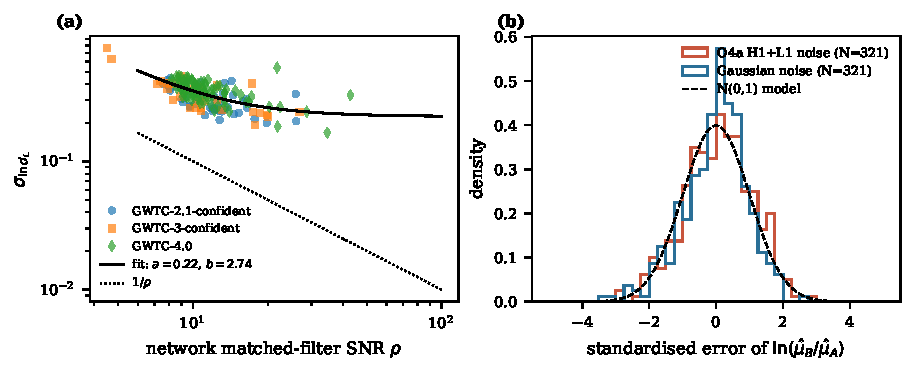
\includegraphics[width=\linewidth]{fig_realdata.pdf}
\caption{Real-data calibration and validation. (a) Log-distance uncertainty versus network matched-filter SNR for 167 confident BBH events in GWTC-1 to GWTC-4.0, with the fitted model used in the simulations. (b) Standardized error of the recovered relative magnification for lensed image pairs injected into public O4a H1/L1 strain and into Gaussian noise with the same PSDs. One glitch-contaminated O4a pair ($z=44.5$) lies outside the plotted range.}
\label{fig:realdata}
\end{figure*}

\section{Inference}
\label{sec:inference}
\subsection{Observables}
\label{sec:features}
The target is the absolute magnification $\mu_A$ of the GW image with the larger measured network SNR (image $A$). The image-geometry observables are the radii of images $A$ and $B$ from the observed lens-light center, their separation, opening angle and asymmetry, an Einstein-radius proxy $(r_A+r_B)/2$, the number of resolved images and the normalized radii of any additional images, the light axis ratio, and the image position angles relative to the light major axis. The GW observables are the magnification ratio $\ln(\hat\mu_B/\hat\mu_A)$ and the arrival order ${\rm sign}(\Delta t)$, which together we call the ``$\mu$ ratio'' below; the delay $\ln|\Delta t|$, which carries a time scale; the two SNRs, which are dimensionless but carry the absolute amplitude and hence depend on the source distance; and the two apparent distances. The follow-up observables are the spectroscopic redshifts $z_l$, $z_s$ and $\ln\sigma_v$. Finally, the estimate $\ln\hat\mu_{\rm cosmo}=2[\ln d_L(\hat z_s)-\ln\hat D_{{\rm app},A}]$ uses the measured source redshift with the Planck18 distance--redshift relation.

Table~\ref{tab:inputsets} lists the combinations of observables that we compare; each is named after the observables it contains. Three properties must be distinguished. The image geometry and the $\mu$ ratio are invariant under the mass-sheet transformation of Sec.~\ref{sec:msd}, and the redshifts and $\sigma_v$, a property of the lens galaxy, are unchanged by an external convergence. None of these observables contains a time or distance scale, so an estimator that uses only them cannot learn the distance--redshift relation of the simulations. We call the four combinations built from them scale-free. Adding the delay and the SNRs introduces a time and an amplitude scale. Without redshifts this adds little (Sec.~\ref{sec:information}); with redshifts, an estimator trained on simulations in one cosmology can relate the delay to the time-delay distance and the SNRs to the luminosity distance, so its output depends on that cosmology even though no distance--redshift relation is supplied explicitly. ``GW\,+\,$z$'' and ``All observables'' contain $\hat\mu_{\rm cosmo}$ explicitly. Distance corrections from these four combinations are therefore circular for cosmography.

\begin{table}
\centering\papertablestyle
\caption{Combinations of observables. ``Scale-free'' combinations are invariant under an external mass sheet and contain no time or distance scale. ``$\mu$ ratio'': the GW magnification ratio $\ln(\hat\mu_B/\hat\mu_A)$ and the arrival order ${\rm sign}(\Delta t)$.}
\label{tab:inputsets}
\begin{tabularx}{\columnwidth}{@{}lLc@{}}
\toprule
Name & Observables & Scale-free \\
\midrule
GW only & $\mu$ ratio, $\ln|\Delta t|$, SNRs, apparent distances & no \\
GW\,+\,$z$ & GW only + $z_l$, $z_s$, $\sigma_v$ + $\hat\mu_{\rm cosmo}$ & no \\
Geometry & image geometry relative to the lens-light center, light shape & yes \\
Geometry\,+\,$z,\sigma_v$ & Geometry + $z_l$, $z_s$, $\sigma_v$ & yes \\
Geometry\,+\,$\mu$ ratio & Geometry + $\ln(\hat\mu_B/\hat\mu_A)$, ${\rm sign}(\Delta t)$ & yes \\
Geometry\,+\,$\mu$ ratio\,+\,$z,\sigma_v$ & the above + $z_l$, $z_s$, $\sigma_v$ & yes \\
Geometry\,+\,$\mu$ ratio\,+\,$\Delta t$, SNR & Geometry\,+\,$\mu$ ratio + $\ln|\Delta t|$, SNRs & no \\
Geometry\,+\,$\mu$ ratio\,+\,$\Delta t$, SNR\,+\,$z,\sigma_v$ & the above + $z_l$, $z_s$, $\sigma_v$ & no \\
All observables & all of the above + apparent distances, $\hat\mu_{\rm cosmo}$ & no \\
\bottomrule
\end{tabularx}
\end{table}

\subsection{Estimators and their uncertainties}
We use two estimators that are constructed (trained) from simulated events. The first is gradient-boosted decision trees in the histogram-based implementation of \textsc{scikit-learn} \citep[hereafter HistGB;][]{pedregosa2011scikit}, trained to predict directly the 5th, 50th and 95th percentiles of $\ln\mu_A$ given the inputs (quantile regression). These percentile estimates need not contain the truth 90\% of the time, so we calibrate them with conformalized quantile regression \citep[CQR;][]{romano2019cqr}. On a separate set of simulated events (the calibration set) we compute for each event how far the true value $y_i$ lies outside its predicted interval, $s_i=\max(\hat q_{05,i}-y_i,\,y_i-\hat q_{95,i})$ (negative if inside), and then widen or narrow all intervals by the value of $s$ that 90\% of the calibration events do not exceed (the $\lceil(n+1)0.9\rceil$-th smallest of the $n$ values). This guarantees 90\% coverage on average over events drawn from the same population as the calibration set, without assuming a Gaussian error distribution. The correction is computed either once for all events (global calibration) or separately within groups of events \citep{vovk2005algorithmic}. The groups are defined either by observed quantities---the number of resolved images or bins of the predicted magnification---or by the true lens family. The latter is a diagnostic only, because the family of a real lens is not known; as an alternative that does not need it, we also calibrate every event on the EPL+shear calibration events alone. Coverage estimates are quoted with binomial uncertainties where they are compared with the nominal level. All simulated events are independent. For each family they are divided at random into 60\% for training, 20\% for calibration and 20\% for testing, on which all results are quoted, and we repeat this with five different random divisions (three for experiments that mix families). Up to 60\,000 selected events per family and scenario are used.

The second estimator is neural posterior estimation \citep[NPE;][]{papamakarios2016fast}, the simulation-based method that has also been used for rapid GW parameter estimation \citep{dax2021neuralposterior}. A neural network---a conditional normalizing flow with spline transformations \citep{durkan2019nsf}, implemented in \textsc{zuko} \citep{rozet2022zuko}---is trained on simulated events to represent the posterior density $p(\ln\mu_A\,|\,\boldsymbol x)$ of the magnification given the inputs $\boldsymbol x$. The posterior median provides the point estimate. We check calibration with the coverage of central intervals at several levels and with the probability integral transform (PIT), the posterior probability below the true value, which is uniformly distributed over events when the posteriors are calibrated.

As a reference without event information we use a prior-only predictor that ignores the event data and returns the percentiles of $\ln\mu_A$ in the training events of the same family. We also evaluate three closed-form estimators: the SIS asymmetry inversion (Eq.~(\ref{eq:sis})), the SIS inversion of the measured relative magnification, and $\hat\mu_{\rm cosmo}$. We report the median relative error $|\hat\mu-\mu|/\mu$, the mean absolute error (MAE) of $\mu_A$, the fraction of events with relative error below 10\%, and the interval coverage (the fraction of events whose true value lies inside the interval) and mean log-width.

\section{Results}
\label{sec:results}
\subsection{Selected populations}
Of the simulated lens systems, 51\% (SIS) and 42--50\% (elliptical families) yield a resolved, detected image pair for ET, and 1.0--1.2\% for the O5-like network (Fig.~\ref{fig:population}). ET pairs have median source redshift $z_s\approx2.7$, median delay of about 54\,d and a median magnification $\mu_A\approx2.5$ of image $A$ (the image with the larger measured SNR). Because the O5-like network must detect both images, its sample is strongly affected by magnification bias. Its pairs lie at lower redshift ($z_s\approx1.9$), are more strongly magnified (median $\mu_A=4.3$--5.2) and contain quadruple-image systems in 33--39\% of the elliptical cases, compared with 5--7\% for ET. These fractions agree with earlier forecasts of a large quad fraction among magnification-selected lensed BBHs \citep{li2018statistical,wierda2021beyond}. Image $A$ is the saddle-point image in 14--20\% of ET pairs and 28--37\% of O5 pairs, because antenna patterns differ between arrival times.

\begin{figure*}
\centering
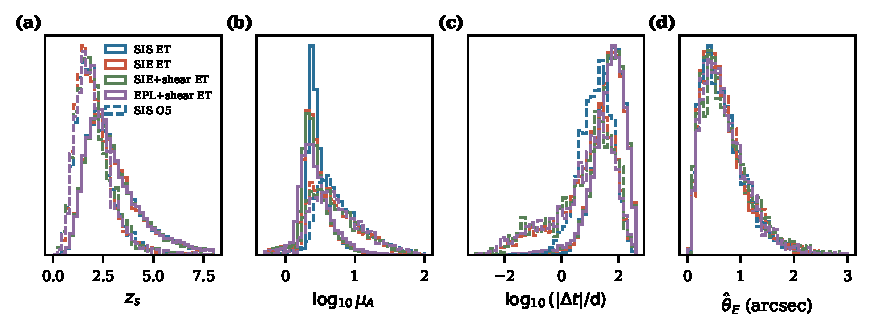
\includegraphics[width=\linewidth]{fig_population.pdf}
\caption{Selected lensed pairs for ET (solid) and the O5-like network (dashed): source redshift, magnification of image $A$ (larger measured SNR), time delay and Einstein-radius proxy, per lens family.}
\label{fig:population}
\end{figure*}

\subsection{Information content of the observables}
\label{sec:information}
Table~\ref{tab:inputs} and Fig.~\ref{fig:inputs} compare the combinations of observables for HistGB estimators simulated and analyzed with the same lens model (in-family), and for one NPE trained on all four lens models. Four results stand out.

\emph{Image geometry dominates.} For ET, geometry alone gives median relative errors of 3.2, 7.3, 11.6 and 19.9\% for SIS, SIE, SIE+shear and EPL+shear lenses, against 19--32\% for the prior-only predictor. Adding the redshifts and velocity dispersion does not help (Geometry\,+\,$z,\sigma_v$), because the image configuration already fixes the dimensionless source position, and $\sigma_v$ with 10\% errors constrains the Einstein radius less precisely than the image positions do. The error grows with the number of unobserved lens degrees of freedom: external shear and, above all, the radial slope of the EPL family change the magnification at fixed image configuration.

\emph{The dimensionless GW observables are complementary.} GW data alone give 7.7\% for SIS---where the relative magnification fixes $y$ through Eq.~(\ref{eq:sis})---but 21--26\% for the elliptical families. Combined with geometry, the GW relative magnification and arrival order alone (Geometry\,+\,$\mu$ ratio) reduce the SIE+shear error from 11.6 to 10.2\% and the EPL+shear error from 19.9 to 18.8\%. These inputs are invariant under the mass-sheet transformation and contain no distance scale; this is the scale-free benchmark of our study.

\emph{The delay and the SNRs add information only through the distance scale.} Adding $\ln|\Delta t|$ and the two SNRs without redshifts (Geometry\,+\,$\mu$ ratio\,+\,$\Delta t$, SNR) changes the errors by at most 0.7 percentage points. With redshifts, however, adding only the delay to Geometry\,+\,$\mu$ ratio\,+\,$z,\sigma_v$ improves the EPL+shear error from 18.7 to 16.7\%, whereas adding only the SNRs leaves it at 18.2\%; all dimensional inputs together give 16.4\%. The neural posterior estimator exploits this much more: with Geometry\,+\,$\mu$ ratio\,+\,$\Delta t$, SNR\,+\,$z,\sigma_v$ it reaches 1.7, 5.9, 9.7 and 13.6\%, against 3.4, 7.2, 10.6 and 19.8\% with the scale-free Geometry\,+\,$\mu$ ratio\,+\,$z,\sigma_v$ inputs. The reason is that $\Delta t=(1+z_l)D_{\Delta t}\Delta\phi/c$, so the delay, the redshifts and the simulated cosmology fix the Fermat-potential difference, which constrains the radial slope that geometry leaves free. This information is real only if the distance scale is known. Table~\ref{tab:response} quantifies the dependence. Rescaling all distances by $1/h$ at fixed redshift, as a Hubble constant $h$ times the simulated one would, shifts the Geometry\,+\,$\mu$ ratio\,+\,$\Delta t$, SNR\,+\,$z,\sigma_v$ NPE estimate by ${\rm d}\ln\hat\mu/{\rm d}\ln h=0.69$ for ET and 0.44 for O5, so a 10\% error in the assumed $H_0$ biases the magnification by 7 (4) percent. Scale-free estimators are unaffected to numerical precision. The same NPE estimates respond to an external mass sheet with ${\rm d}\ln\hat\mu/{\rm d}\ln\lambda=-0.69$, whereas the truth scales as $-2$: they partly absorb $\kappa_{\rm ext}$ by misattributing the shorter delay to a steeper lens, but cannot correct for it. HistGB estimates respond less to these transformations (${\rm d}\ln\hat\mu/{\rm d}\ln h=0.13$ for ET), because decision trees predict constant values outside the range of their training data; they are therefore less sensitive to the assumed cosmology but gain correspondingly less from it.

\emph{Known redshift plus cosmology is not competitive on its own.} Inverting the apparent distance with the source redshift gives 41\% errors for all families, because the inclination--distance degeneracy calibrated on real events (Sec.~\ref{sec:realdata}) limits the apparent distance of a single image to $\sigma_{\ln D}\gtrsim0.22$, i.e. $\gtrsim45$ percent in magnification. Section~\ref{sec:pe} shows that full parameter estimation of both images reduces this floor. Closed-form SIS inversions perform well only when the SIS model is correct and degrade to 21--43\% for the elliptical families. A flexible estimator trained on a realistic lens prior is therefore essential.

For the O5-like network all errors are larger (Table~\ref{tab:inputs}b): 10.7, 16.2, 21.9 and 27.9\% with geometry and 10.8, 14.8, 18.8 and 25.5\% with Geometry\,+\,$\mu$ ratio. This is because magnification bias selects highly magnified, near-caustic configurations. The errors stop decreasing above about $10^4$ training events (Fig.~\ref{fig:learning} in Appendix~\ref{app:extra}), so the ET results are not limited by sample size; the smaller O5 samples (1500--3000 per family) cost about 1--2 percentage points.

\begin{table*}
\centering\papertablestyle
\caption{Median relative error $|\hat\mu_A-\mu_A|/\mu_A$ (percent) of the magnification of image $A$ (larger measured SNR). Parentheses: empirical coverage of the conformal 90\% intervals (binomial standard error per division 0.003 for ET and 0.01--0.02 for O5). Top: closed-form estimators. Middle: HistGB trained and tested on the same family, means over five random divisions into training, calibration and test events (standard deviation between divisions below 0.3 percentage points for ET and 1.5 for O5). Bottom: one NPE trained on all four families, with intervals calibrated per true family, which is not possible for real lenses (see Table~\ref{tab:calibration}). Prior only: percentiles of the simulated population, ignoring the event data. $^\dagger$Scale-free combinations (Table~\ref{tab:inputsets}).}
\label{tab:inputs}
\textbf{(a) ET}\par\smallskip
\begin{tabular*}{\linewidth}{@{\extracolsep{\fill}}lcccc@{}}
\toprule
Observables & SIS & SIE & SIE+shear & EPL+shear \\
\midrule
SIS analytic (geometry) & 3.3 & 21.0 & 23.8 & 32.9 \\
SIS analytic ($\mu$ ratio) & 8.7 & 33.0 & 36.5 & 42.5 \\
$z_s$ + cosmology & 40.8 & 41.6 & 41.4 & 41.3 \\
\midrule
Prior only$^\dagger$ & 18.7 (0.90) & 24.3 (0.90) & 25.0 (0.90) & 31.6 (0.90) \\
GW only & 7.7 (0.90) & 21.4 (0.90) & 21.9 (0.90) & 25.8 (0.90) \\
GW\,+\,$z$ & 6.7 (0.90) & 16.9 (0.90) & 17.3 (0.90) & 19.4 (0.90) \\
Geometry$^\dagger$ & 3.2 (0.90) & 7.3 (0.90) & 11.6 (0.90) & 19.9 (0.90) \\
Geometry\,+\,$z,\sigma_v$$^\dagger$ & 3.2 (0.90) & 7.3 (0.90) & 11.6 (0.90) & 19.8 (0.90) \\
Geometry\,+\,$\mu$ ratio$^\dagger$ & 3.0 (0.90) & 6.9 (0.90) & 10.2 (0.90) & 18.8 (0.90) \\
Geometry\,+\,$\mu$ ratio\,+\,$z,\sigma_v$$^\dagger$ & 3.0 (0.90) & 7.0 (0.90) & 10.2 (0.90) & 18.7 (0.90) \\
Geometry\,+\,$\mu$ ratio\,+\,$\Delta t$, SNR & 2.9 (0.90) & 6.9 (0.90) & 9.9 (0.90) & 18.1 (0.90) \\
Geometry\,+\,$\mu$ ratio\,+\,$\Delta t$, SNR\,+\,$z,\sigma_v$ & 2.7 (0.90) & 6.9 (0.90) & 9.9 (0.90) & 16.4 (0.90) \\
All observables & 2.7 (0.90) & 6.9 (0.90) & 10.0 (0.90) & 15.6 (0.90) \\
\midrule
NPE: GW only & 9.7 (0.90) & 22.4 (0.90) & 23.9 (0.90) & 27.5 (0.89) \\
NPE: Geometry$^\dagger$ & 3.4 (0.90) & 7.3 (0.90) & 11.9 (0.89) & 20.9 (0.90) \\
NPE: Geometry\,+\,$\mu$ ratio$^\dagger$ & 3.3 (0.90) & 6.8 (0.90) & 10.6 (0.89) & 19.6 (0.89) \\
NPE: Geometry\,+\,$\mu$ ratio\,+\,$z,\sigma_v$$^\dagger$ & 3.4 (0.90) & 7.2 (0.90) & 10.6 (0.89) & 19.8 (0.90) \\
NPE: Geometry\,+\,$\mu$ ratio\,+\,$\Delta t$, SNR & 3.3 (0.90) & 6.7 (0.90) & 10.2 (0.89) & 18.8 (0.89) \\
NPE: Geometry\,+\,$\mu$ ratio\,+\,$\Delta t$, SNR\,+\,$z,\sigma_v$ & 1.7 (0.89) & 5.9 (0.90) & 9.7 (0.90) & 13.6 (0.90) \\
NPE: All observables & 1.8 (0.90) & 6.0 (0.90) & 9.8 (0.90) & 13.8 (0.90) \\
\bottomrule
\end{tabular*}
\par\bigskip\textbf{(b) O5-like network}\par\smallskip
\begin{tabular*}{\linewidth}{@{\extracolsep{\fill}}lcccc@{}}
\toprule
Observables & SIS & SIE & SIE+shear & EPL+shear \\
\midrule
SIS analytic (geometry) & 9.7 & 45.3 & 54.5 & 58.0 \\
SIS analytic ($\mu$ ratio) & 34.2 & 59.6 & 63.7 & 63.2 \\
$z_s$ + cosmology & 46.0 & 49.2 & 53.1 & 50.4 \\
\midrule
Prior only$^\dagger$ & 49.7 (0.91) & 53.5 (0.89) & 52.9 (0.91) & 55.8 (0.90) \\
GW only & 29.5 (0.91) & 35.3 (0.90) & 35.4 (0.90) & 34.8 (0.88) \\
GW\,+\,$z$ & 19.0 (0.92) & 26.5 (0.89) & 26.8 (0.90) & 29.2 (0.90) \\
Geometry$^\dagger$ & 10.7 (0.90) & 16.2 (0.90) & 21.9 (0.91) & 27.9 (0.88) \\
Geometry\,+\,$z,\sigma_v$$^\dagger$ & 10.7 (0.90) & 16.3 (0.89) & 23.4 (0.91) & 27.9 (0.91) \\
Geometry\,+\,$\mu$ ratio$^\dagger$ & 10.8 (0.90) & 14.8 (0.89) & 18.8 (0.90) & 25.5 (0.90) \\
Geometry\,+\,$\mu$ ratio\,+\,$z,\sigma_v$$^\dagger$ & 10.5 (0.90) & 15.0 (0.89) & 19.4 (0.90) & 25.7 (0.90) \\
Geometry\,+\,$\mu$ ratio\,+\,$\Delta t$, SNR & 9.9 (0.90) & 15.4 (0.90) & 17.9 (0.90) & 24.8 (0.89) \\
Geometry\,+\,$\mu$ ratio\,+\,$\Delta t$, SNR\,+\,$z,\sigma_v$ & 8.8 (0.91) & 14.7 (0.90) & 18.3 (0.89) & 24.6 (0.90) \\
All observables & 8.8 (0.91) & 15.7 (0.90) & 17.7 (0.90) & 24.2 (0.89) \\
\midrule
NPE: GW only & 29.3 (0.91) & 36.3 (0.88) & 39.7 (0.89) & 36.6 (0.89) \\
NPE: Geometry$^\dagger$ & 11.3 (0.89) & 14.3 (0.92) & 22.6 (0.90) & 24.8 (0.90) \\
NPE: Geometry\,+\,$\mu$ ratio$^\dagger$ & 10.4 (0.89) & 12.4 (0.90) & 18.0 (0.90) & 27.2 (0.91) \\
NPE: Geometry\,+\,$\mu$ ratio\,+\,$z,\sigma_v$$^\dagger$ & 10.6 (0.89) & 13.1 (0.89) & 17.3 (0.89) & 27.6 (0.91) \\
NPE: Geometry\,+\,$\mu$ ratio\,+\,$\Delta t$, SNR & 11.4 (0.91) & 12.3 (0.91) & 20.1 (0.90) & 26.2 (0.92) \\
NPE: Geometry\,+\,$\mu$ ratio\,+\,$\Delta t$, SNR\,+\,$z,\sigma_v$ & 7.2 (0.90) & 10.7 (0.91) & 15.0 (0.92) & 21.3 (0.94) \\
NPE: All observables & 7.3 (0.91) & 11.1 (0.89) & 15.4 (0.92) & 19.4 (0.93) \\
\bottomrule
\end{tabular*}
\end{table*}

\begin{table*}
\centering\papertablestyle
\caption{Response of the predicted magnification to an external mass sheet ($\lambda=1-\kappa_{\rm ext}$; the truth scales as ${\rm d}\ln\mu/{\rm d}\ln\lambda=-2$) and to a distance scale $1/h$ at fixed redshift (the truth is unchanged). Slopes from $\pm10$ percent transformations of the fixed test systems.}
\label{tab:response}
\begin{tabular*}{\linewidth}{@{\extracolsep{\fill}}llcccc@{}}
\toprule
 & & \multicolumn{2}{c}{${\rm d}\ln\hat\mu/{\rm d}\ln\lambda$} & \multicolumn{2}{c}{${\rm d}\ln\hat\mu/{\rm d}\ln h$} \\
Scen. & Observables & HistGB & NPE & HistGB & NPE \\
\midrule
ET & Geometry\,+\,$\mu$ ratio\,+\,$z,\sigma_v$ & +0.00 & +0.00 & +0.00 & +0.00 \\
ET & Geometry\,+\,$\mu$ ratio\,+\,$\Delta t$, SNR & -0.03 & -0.04 & +0.03 & +0.04 \\
ET & Geometry\,+\,$\mu$ ratio\,+\,$\Delta t$\,+\,$z,\sigma_v$ & -0.10 & -- & +0.10 & -- \\
ET & Geometry\,+\,$\mu$ ratio\,+\,SNR\,+\,$z,\sigma_v$ & -0.03 & -- & +0.03 & -- \\
ET & Geometry\,+\,$\mu$ ratio\,+\,$\Delta t$, SNR\,+\,$z,\sigma_v$ & -0.13 & -0.69 & +0.13 & +0.69 \\
ET & All observables & -0.21 & -0.71 & +0.21 & +0.71 \\
O5 & Geometry\,+\,$\mu$ ratio\,+\,$z,\sigma_v$ & +0.00 & -0.00 & +0.00 & -0.00 \\
O5 & Geometry\,+\,$\mu$ ratio\,+\,$\Delta t$, SNR & -0.08 & -0.15 & +0.09 & +0.14 \\
O5 & Geometry\,+\,$\mu$ ratio\,+\,$\Delta t$\,+\,$z,\sigma_v$ & -0.03 & -- & +0.03 & -- \\
O5 & Geometry\,+\,$\mu$ ratio\,+\,SNR\,+\,$z,\sigma_v$ & -0.08 & -- & +0.08 & -- \\
O5 & Geometry\,+\,$\mu$ ratio\,+\,$\Delta t$, SNR\,+\,$z,\sigma_v$ & -0.14 & -0.43 & +0.13 & +0.44 \\
O5 & All observables & -0.30 & -0.56 & +0.30 & +0.56 \\
\bottomrule
\end{tabular*}
\end{table*}

\begin{figure*}
\centering
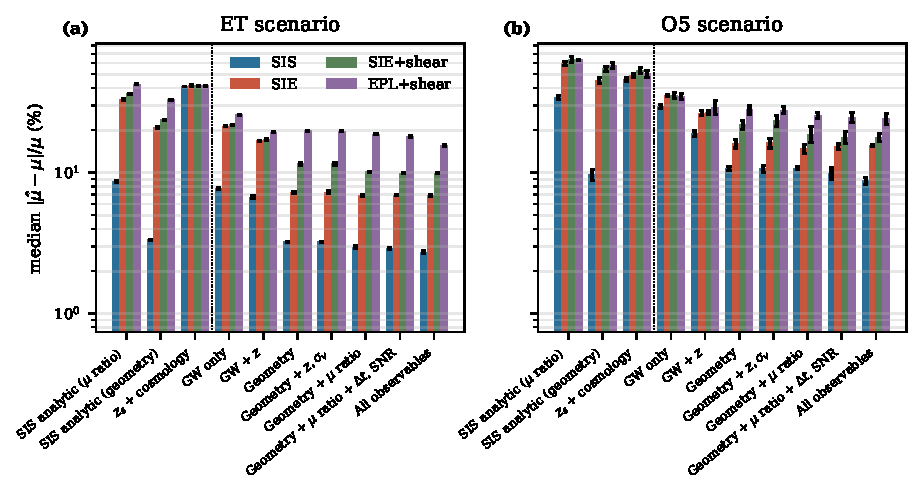
\includegraphics[width=\linewidth]{fig_inputs.pdf}
\caption{Median relative magnification error by combination of observables and lens family (in-family training; error bars: standard deviation over five random divisions). Left of the dotted line: closed-form estimators.}
\label{fig:inputs}
\end{figure*}

\subsection{Near-caustic configurations}
Errors grow rapidly with magnification (Fig.~\ref{fig:tail}). With the scale-free Geometry\,+\,$\mu$ ratio inputs for ET, the median relative error rises from 2--13\% at $2<\mu_A<3$ to 10--34\% at $5<\mu_A<10$ and 44--57\% at $\mu_A>20$. This is consistent with $\delta\ln|\mu|=-\operatorname{tr}(A^{-1}\delta A)$, whose dominant term grows in proportion to $|\mu|$ as an image approaches a critical curve, so that a given astrometric and model uncertainty produces larger magnification errors; the near-linear trend is a result for our lens populations and error model rather than a general law. The rise at $\mu_A<2$ reflects demagnified saddle images that are brighter in SNR only because of the antenna pattern. Intervals calibrated over the whole population contain the truth too rarely in the high-magnification tail (coverage 0.65--0.80 at $10<\mu_A\le20$ and 0.44--0.57 above 20), even though they cover 90\% of events overall (Sec.~\ref{sec:calibration}). Neural posterior estimation with the same scale-free inputs reduces the tail errors only moderately, to 30--46\% at $\mu_A>20$. With the delay and redshifts (Geometry\,+\,$\mu$ ratio\,+\,$\Delta t$, SNR\,+\,$z,\sigma_v$) the tail errors fall to 6--21\%: once $D_{\Delta t}$ is specified, the measured delay constrains the Fermat-potential difference, which is complementary to the image positions and the magnification ratio. This gain therefore relies on the assumed cosmology and on $\kappa_{\rm ext}=0$.

\begin{figure*}
\centering
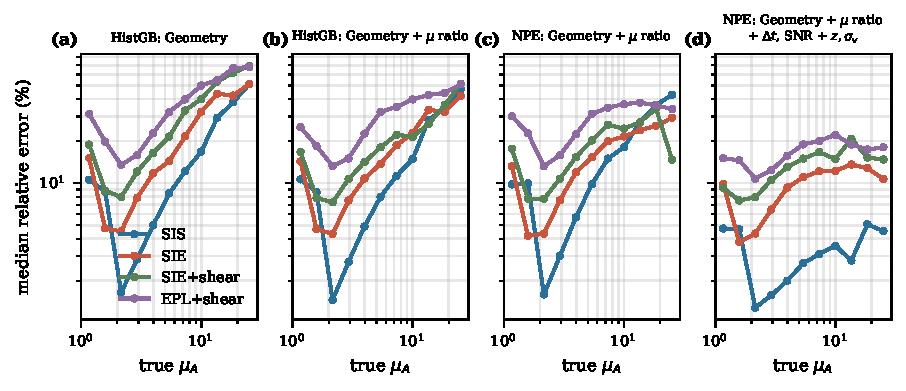
\includegraphics[width=\linewidth]{fig_tail.pdf}
\caption{Median relative error versus true magnification for ET. (a), (b) In-family HistGB models with Geometry and the scale-free Geometry\,+\,$\mu$ ratio inputs (test events of one random division); (c), (d) NPE trained on all families with the scale-free Geometry\,+\,$\mu$ ratio and the scale-dependent Geometry\,+\,$\mu$ ratio\,+\,$\Delta t$, SNR\,+\,$z,\sigma_v$ inputs.}
\label{fig:tail}
\end{figure*}

\subsection{Calibration of the uncertainties}
\label{sec:calibration}
Within a single lens family, CQR intervals achieve the nominal coverage for every combination of observables and both scenarios (0.88--0.92; Table~\ref{tab:inputs}). A single model trained on all four families is almost as accurate as the in-family models (3.4, 7.1, 11.0 and 20.0\% with Geometry\,+\,$\mu$ ratio for ET), but a single conformal correction for all families is wrong for each of them. It over-covers SIS and SIE (0.95--0.97) and under-covers EPL+shear (0.75), because the families have different error distributions (Table~\ref{tab:calibration}, Fig.~\ref{fig:coverage}a). Calibrating separately per true family restores 0.90 coverage in every family, but the true family of a real lens is not known. Calibration groups defined by observables do not reproduce it: grouping by the number of images or by the predicted magnification leaves the EPL+shear coverage at 0.75--0.76, because these observables hardly distinguish the families. What does work without a family label is to calibrate on the most flexible family alone. Conformal correction computed on the EPL+shear calibration events gives coverage of at least 0.90 in every family, at the price of 40\% wider intervals and over-coverage (0.98--0.99) for the simpler families. The O5 results are similar (Table~\ref{tab:calibration}b).

The conformal guarantee holds on average over the population, or within any group of events defined by \emph{observed} quantities, but not within groups defined by the unobserved true magnification. We therefore also calibrated in-family models in five bins of the \emph{predicted} magnification (Fig.~\ref{fig:coverage}b). By construction this restores 90\% coverage in every predicted-magnification bin, but coverage in bins of the true magnification hardly changes: averaged over families it is 0.84, 0.75 and 0.54 for true $\mu_A$ in $(5,10]$, $(10,20]$ and above 20 for ET, against 0.82, 0.73 and 0.51 with a single calibration for all magnifications. Truly near-caustic events are under-covered because, given the measurement noise, they are partly indistinguishable from moderately magnified configurations, and the estimators pull them towards typical magnifications. This is a remaining failure of all calibrated estimators in our study, not one that predicted-magnification calibration solves. Interval widths must therefore be interpreted as conditional on the observables, and analyses that select events by high inferred magnification should account for this regression to the mean.

NPE provides the posterior distribution of $\ln\mu_A$, marginalized over all other lens and source parameters. Trained once on all four families with the scale-free Geometry\,+\,$\mu$ ratio inputs for ET, the posterior median reaches 3.3, 6.8, 10.6 and 19.6\%, comparable to the in-family HistGB models (3.0, 6.9, 10.2 and 18.8\%) without access to the family label. Its posteriors before any interval correction are calibrated over the whole population but not per family (coverage 0.94, 0.97, 0.92 and 0.76; Fig.~\ref{fig:coverage}c): the network learns an average error distribution, exactly like the global conformal correction. The same calibration choices apply. Per-true-family recalibration restores 0.89--0.90 in every family; observable groups do not; EPL+shear calibration gives 0.89--0.99. Conformal recalibration adjusts the end points of the 90\% interval only and does not by itself certify the rest of the posterior density.

\begin{table*}
\centering\papertablestyle
\caption{Coverage of the 90\% intervals per lens family for one model trained on all four families with Geometry\,+\,$\mu$ ratio inputs, for different conformal calibrations. ``Width'' is the mean width of $\ln\mu_A$ intervals over all families. The true-family calibration is a diagnostic only, because the family of a real lens is unknown. HistGB: means over three random divisions; binomial standard errors are below 0.006 (ET) and 0.02 (O5).}
\label{tab:calibration}
\textbf{(a) ET}\par\smallskip
\begin{tabular*}{\linewidth}{@{\extracolsep{\fill}}llccccc@{}}
\toprule
Estimator & Calibration & SIS & SIE & SIE+shear & EPL+shear & width \\
\midrule
HistGB & global & 0.95 & 0.97 & 0.91 & 0.75 & 0.67 \\
HistGB & image multiplicity & 0.95 & 0.97 & 0.92 & 0.76 & 0.67 \\
HistGB & predicted $\mu$ & 0.95 & 0.97 & 0.91 & 0.75 & 0.68 \\
HistGB & EPL+shear only & 0.99 & 0.99 & 0.98 & 0.90 & 0.94 \\
HistGB & true family (diagnostic) & 0.90 & 0.90 & 0.90 & 0.90 & 0.68 \\
\midrule
NPE & global & 0.94 & 0.97 & 0.92 & 0.76 & 0.65 \\
NPE & image multiplicity & 0.94 & 0.97 & 0.92 & 0.76 & 0.65 \\
NPE & predicted $\mu$ & 0.94 & 0.97 & 0.92 & 0.76 & 0.65 \\
NPE & EPL+shear only & 0.99 & 0.99 & 0.98 & 0.89 & 0.91 \\
NPE & true family (diagnostic) & 0.90 & 0.90 & 0.89 & 0.89 & 0.66 \\
\bottomrule
\end{tabular*}
\par\bigskip\textbf{(b) O5-like network}\par\smallskip
\begin{tabular*}{\linewidth}{@{\extracolsep{\fill}}llccccc@{}}
\toprule
Estimator & Calibration & SIS & SIE & SIE+shear & EPL+shear & width \\
\midrule
HistGB & global & 0.92 & 0.92 & 0.87 & 0.81 & 1.13 \\
HistGB & image multiplicity & 0.92 & 0.92 & 0.88 & 0.82 & 1.13 \\
HistGB & predicted $\mu$ & 0.92 & 0.91 & 0.88 & 0.81 & 1.15 \\
HistGB & EPL+shear only & 0.95 & 0.96 & 0.95 & 0.90 & 1.38 \\
HistGB & true family (diagnostic) & 0.88 & 0.90 & 0.88 & 0.90 & 1.11 \\
\midrule
NPE & global & 0.94 & 0.93 & 0.91 & 0.80 & 1.01 \\
NPE & image multiplicity & 0.92 & 0.94 & 0.92 & 0.82 & 1.02 \\
NPE & predicted $\mu$ & 0.94 & 0.94 & 0.91 & 0.80 & 1.02 \\
NPE & EPL+shear only & 0.99 & 0.98 & 0.96 & 0.91 & 1.43 \\
NPE & true family (diagnostic) & 0.89 & 0.90 & 0.90 & 0.91 & 0.98 \\
\bottomrule
\end{tabular*}
\end{table*}

\begin{figure*}
\centering
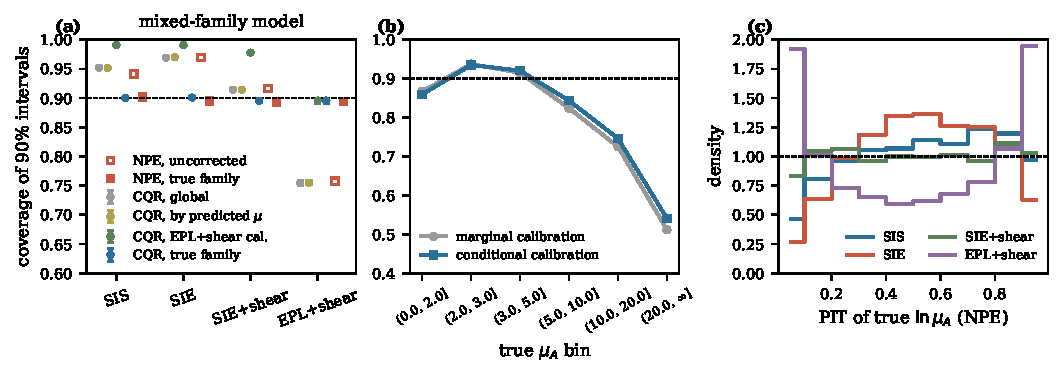
\includegraphics[width=\linewidth]{fig_coverage.pdf}
\caption{Calibration of the 90\% intervals for ET (Geometry\,+\,$\mu$ ratio inputs). (a) Coverage per family for a HistGB model trained on all families with global, predicted-magnification, EPL+shear-only and true-family conformal calibration (error bars: scatter between random divisions), and for neural posterior estimation (raw and recalibrated per true family). (b) Coverage in bins of true magnification for a single calibration (``marginal'') and for calibration within bins of predicted magnification (``conditional''); in-family models, mean over families and three random divisions. (c) Histograms of the PIT (posterior probability below the true value) for the NPE; a flat histogram indicates calibrated posteriors.}
\label{fig:coverage}
\end{figure*}

\subsection{Wrong lens-model assumptions}
\label{sec:transfer}
Fig.~\ref{fig:transfer} shows models trained on one family and applied to another. Training on SIS lenses---the default assumption of many lensed-GW forecasts---is the worst choice. Applied to elliptical lenses it gives 21--31\% errors with 90\% intervals covering only 20--27\% of the true values: the SIS prior produces biased estimates with underestimated uncertainties. As in neural lens modeling of galaxy--galaxy lenses, the simulated training population acts as a prior, and differences between it and the true population bias the inference \citep{wagnercarena2021hierarchical,park2021largescale}. Conversely, the most flexible EPL+shear prior transfers to the simpler families at a moderate accuracy cost (9.4--13.0\% instead of 3.0--10.3\% in-family) and conservative coverage (0.96--0.98). The SIE and SIE+shear priors transfer well to each other and to SIS, but under-cover EPL+shear lenses (0.48 and 0.61). When SIS, SIE or SIE+shear lenses are omitted from the training set of a model trained on several families, the intervals still cover 91--97\% of their true values, at a moderate accuracy cost (for SIS, 3.4 rises to 6.6\%), whereas omitting EPL+shear lenses yields 22\% errors and coverage 0.55. The radial density slope is thus the dominant lens-model systematic: training sets must include slope variations comparable to those of real lenses, and calibration should use the broadest plausible lens population. This conservative transfer is established only among our four families; real lenses with structure outside the EPL+shear family can still be misdescribed.

\begin{figure*}
\centering
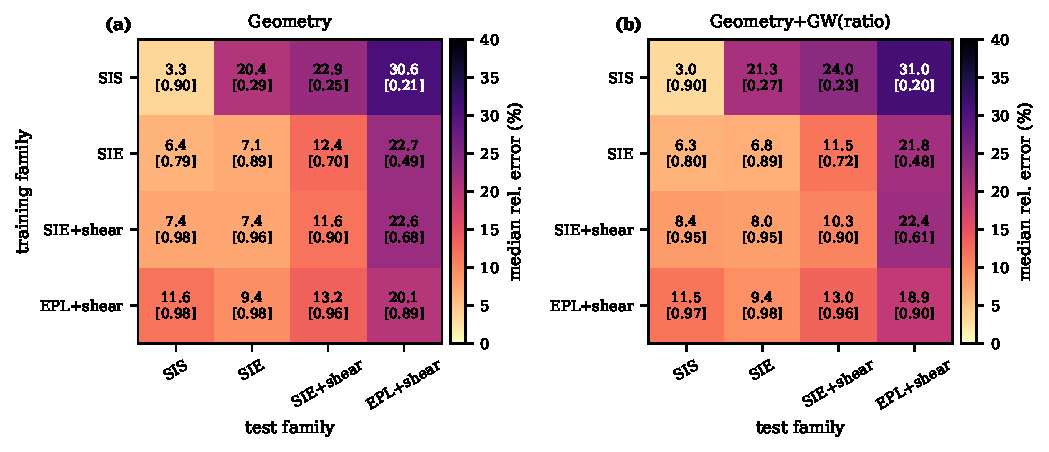
\includegraphics[width=\linewidth]{fig_transfer.pdf}
\caption{Transfer between lens families for ET. Cells give the median relative error (percent) and, in brackets, the coverage of the 90\% intervals, for models trained on the row family and tested on the column family.}
\label{fig:transfer}
\end{figure*}

\subsection{Sky localization}
The GW relative magnification requires the antenna response of both images, and hence the sky position, polarization and inclination. With the sky and orientation uncertainties expected for ET alone, the median error of the GW-only SIS estimate is 7.7\%; with the sky position known (for example from the identified host galaxy) it falls to 3.9\%. Combined with geometry, known sky improves the Geometry\,+\,$\mu$ ratio errors from 10.2 to 8.1\% for SIE+shear and from 18.8 to 17.3\% for EPL+shear. Host identification therefore also sharpens the GW relative magnification \citep{hannuksela2020localizing,wempe2022lensing}. Because the main benchmark assumes an identified host, its estimated-sky GW errors are conservative; for the single ET detector, fixing the sky position to that of the host also avoids the poorly explored solutions found in our free-sky joint PE (Sec.~\ref{sec:jointpe}).

\subsection{Luminosity distance}
\label{sec:distance}
The magnification correction gives $\hat d_L=\hat D_{{\rm app},A}\,\hat\mu_A^{1/2}$, evaluated event by event, so any correlation between the two estimates is retained. For the scale-free observables the magnification estimate does not use the apparent distance, but the two estimates share the SNR and the antenna-response errors of image $A$; evaluating $\hat d_L$ event by event includes this correlation. For ET with Geometry\,+\,$\mu$ ratio inputs the magnification contributes a median $|\delta\ln d_L|$ of 1.5, 3.5, 5.1 and 9.5\% for SIS, SIE, SIE+shear and EPL+shear. The total median error is 22--24\%, almost the same as the 22\% obtained with the true magnification (Fig.~\ref{fig:distance}). For O5 the magnification contributes 5--13\%, against a total of 27--33\%. Under the catalog-calibrated apparent-distance model, magnification inferred from image geometry is therefore not the limiting factor for the distance of a typical lensed BBH; the exception is a strongly magnified image ($\mu\gtrsim10$). This conclusion depends on the apparent-distance error. The catalog-calibrated floor $\sigma_{\ln D}\approx0.22$ reflects current detectors, waveform models and the inclination--distance degeneracy; higher harmonics reduce it for third-generation detectors \citep{liu2024harmonics}, and our joint PE gives ET apparent-distance errors less than half as large (Sec.~\ref{sec:jointpe}). With such errors the magnification term is comparable to the GW term for elliptical lenses.

\begin{figure}
\centering
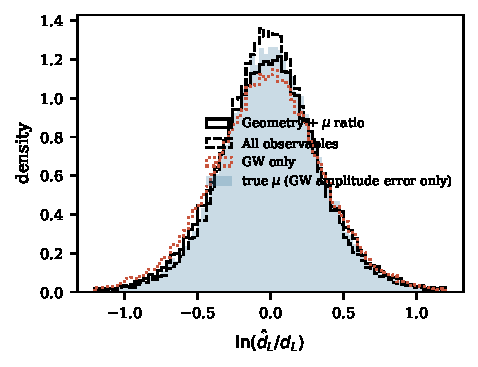
\includegraphics[width=\columnwidth]{fig_distance.pdf}
\caption{Error of the magnification-corrected luminosity distance for ET (all families). The shaded histogram uses the true magnification and shows the GW apparent-distance error alone.}
\label{fig:distance}
\end{figure}

\section{Parameter estimation and Bayesian lens reconstruction}
\label{sec:pe}
The benchmark of Sec.~\ref{sec:results} uses a simplified, SNR-based model of the GW measurements (Sec.~\ref{sec:gwmeas}) and estimators trained on simulations. Here we test both ingredients on a random subset of systems, with equal numbers per lens family and scenario: the SNR-based model against joint Bayesian parameter estimation (PE) of both images from simulated detector data (strain), and the trained estimators against a conventional Bayesian lens reconstruction from comparable observables. The information available to each method is stated explicitly below, because it is not identical.

\subsection{Joint parameter estimation of lensed image pairs}
\label{sec:jointpe}
We drew 15 selected systems per lens family and scenario (120 in total) at random from catalogs generated with the same configuration as the benchmark, excluding the lightest detector-frame binaries whose analysis segment would exceed 256\,s. For each system both images were injected into independent stationary Gaussian noise with the A+/AdV (O5-like) or ET-D power spectral densities, using the \textsc{IMRPhenomXHM} waveform with higher harmonics \citep{garciaquiros2020xhm}, the Morse phase of each image and the antenna patterns at each arrival time. We sampled the joint posterior of the shared source parameters (chirp mass, mass ratio, aligned spins, sky position, polarization, inclination, phase, apparent distance and arrival time of image $A$) and the lensing parameters $\ln(\mu_B/\mu_A)$, the delay and the two Morse indices, with \textsc{bilby} \citep{ashton2019bilby}, the \textsc{dynesty} nested sampler \citep{speagle2020dynesty} and relative binning \citep{zackay2018relbin,krishna2023relbin}, which speeds up the likelihood by expanding each waveform around a reference waveform. In this controlled test the reference is the injected signal; for real data it would be a maximum-likelihood fit. Where the relative-binning log-likelihood exceeds that of the reference by more than 50, which signals a failure of the approximation because the reference lies close to the maximum-likelihood point, we evaluate the exact likelihood instead. This safeguard does not bound the error elsewhere, so we evaluated the exact likelihood on 500 posterior samples of every system whose stored samples allow it (all 60 ET and 52 of the 60 O5 systems; the stored samples of eight early O5 runs lack the phase) and reweighted the samples by the likelihood ratio. For O5 the difference is negligible (posterior shifts of $\ln(\mu_B/\mu_A)$ below $0.03\sigma$). For ET the log-likelihood differences have a typical scatter of 0.27; reweighting shifts the median of $\ln(\mu_B/\mu_A)$ by a median $0.01\sigma$ (at most $0.10\sigma$) and that of $\ln D_{{\rm app},A}$ by $0.03\sigma$ (at most $0.25\sigma$), changes interval widths by less than 10\% for the magnification ratio, and leaves its coverage unchanged. We analyzed every system twice: with a free sky position, as in a GW-only analysis, and with the sky position fixed to that of the host, which is known to sub-arcsecond precision once the lens system is identified in imaging, as the benchmark assumes. The apparent-distance prior is uniform in volume. We used 150 live points and the acceptance-walk method of \textsc{bilby}, with 30 accepted Markov-chain steps for each new live point. For the free-sky ET posteriors, which have several separated solutions, these settings do not explore all of them (see below), which is one reason we base the comparison with the SNR-based model on the known-sky analyses. Each system has its own noise realization, fixed by a seed derived from its identifier, so that the GW-only and GW+EM analyses below see identical data. A run takes of order 10--30 CPU hours.

Fig.~\ref{fig:pe} compares the joint-PE posteriors with the SNR-based model of Sec.~\ref{sec:gwmeas}. With the host sky position, the 90\% intervals of $\ln(\mu_B/\mu_A)$ and of the apparent distance of image $A$ contain the truth for 52 and 50 of the 60 ET systems (coverage $0.87\pm0.04$ and $0.83\pm0.05$, binomial errors), and the free-sky O5 intervals for 55 and 53 of 60 ($0.92\pm0.04$ and $0.88\pm0.04$). The probability integral transforms are consistent with uniform (Kolmogorov--Smirnov $p=0.06$ for ET and $0.09$ for O5), and the difference of Morse indices is identified with posterior probability above 0.5 in all ET and in 59 of 60 O5 systems. For the tested systems the PE uncertainties are smaller than those of the SNR-based model: by a factor 0.91 for $\ln(\mu_B/\mu_A)$ in O5 and 0.41 in ET, and by factors 0.67 and 0.44 for $\ln D_{{\rm app},A}$. In these comparisons the SNR-based model is therefore conservative, especially for ET. The joint PE fixes the source parameters that the two images share, and the higher harmonics break part of the inclination--distance degeneracy that dominates the catalog-calibrated apparent-distance errors, so the median $\sigma_{\ln D}$ is 0.10 for ET rather than 0.24.

Free-sky ET analyses fail in a characteristic way. A single ET site constrains the sky position poorly, and the sky position, the polarization and the Morse phase of each image are partly degenerate. With 150 live points the median sky offset is $56\degr$, the Morse-index difference is identified in only 82\% of systems, and the coverage of $\ln(\mu_B/\mu_A)$ falls to 0.67. With 500 live points the coverage rises only to 0.75, and for the 15 systems whose intervals still miss the truth the posterior favors other sky positions, so these failures are a property of single-site data rather than of the sampler. Fixing the sky position to that of the identified host, which is available whenever the lens is identified, removes them. O5 analyses, with three detectors, are not affected.

As a test of the complete chain from detector data to magnification, we replaced the simulated magnification ratio in the input of the scale-free Geometry\,+\,$\mu$ ratio\,+\,$z,\sigma_v$ NPE by the PE posterior median and kept the per-family conformal calibration of Sec.~\ref{sec:calibration}. The median relative error of $\mu_A$ is 10.5\% for ET with the host sky position (10.8\% with the SNR-based model) and 13.8\% for O5 (17.8\%), with coverage 0.85 and 0.87 for both inputs. The NPE trained with the SNR-based model therefore works with relative magnifications measured by full PE. The SIS intervals under-cover in this subset (0.67--0.73 of 15 systems) for both inputs; these intervals are only a few percent wide, and the test-set coverage for SIS is nominal, so we attribute this to the small sample.

\begin{figure*}
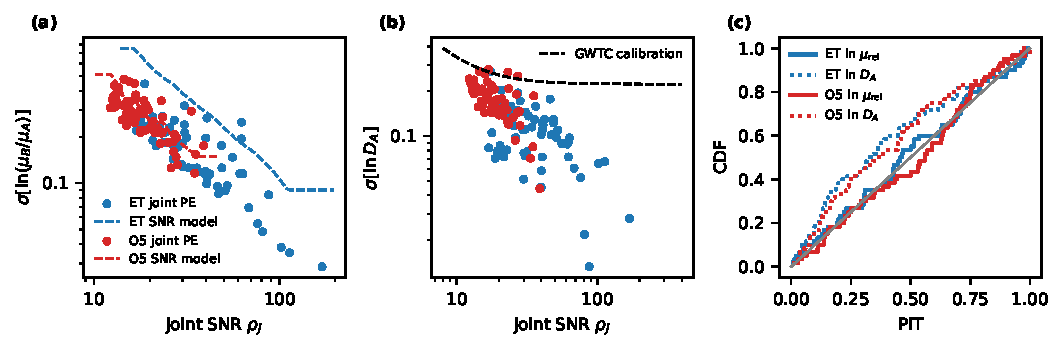
\includegraphics[width=\textwidth]{figures/fig_pe.pdf}
\caption{Joint PE of 120 lensed image pairs from simulated strain. (a) Posterior standard deviation of $\ln(\mu_B/\mu_A)$ versus joint network SNR, with the SNR-based model (dashed). (b) The same for the apparent distance of image $A$, with the GWTC-calibrated error model. (c) Distribution of the probability integral transforms of the truth (diagonal: perfect calibration). ET uses the host sky position, O5 a free sky position.}
\label{fig:pe}
\end{figure*}

\subsection{Bayesian GW+EM lens reconstruction}
\label{sec:gwem}
For the same systems we reconstructed the lens with a conventional likelihood, specified in Appendix~\ref{app:gwemlike}. The lens model is the simulated family (SIS, SIE, SIE+shear or EPL+shear), evaluated with \textsc{lenstronomy}, and its priors are the simulated population distributions: the SLACS-like axis ratio, the log-normal external shear, $\gamma'\sim\mathcal N(2.08,0.15)$ and the $\sigma_v^4$-weighted velocity-dispersion function. The EM likelihood contains the image positions, with the source position integrated out analytically after linearizing the lens equation around each observed image, the lens-light axis ratio and orientation, the velocity dispersion through the SIS normalization, and the lens-light center. The prior of the source position is normalized for each lens as in the simulation; without this normalization the fit favors steep radial profiles (Appendix~\ref{app:gwemlike}). The GW data enter through the joint-PE posterior of Sec.~\ref{sec:jointpe}, summarized by a Gaussian in $\ln(\mu_B/\mu_A)$ after reweighting the samples to remove the distance prior and multiplied by the posterior probabilities of the nine Morse-index combinations, analogous to the effective GW likelihood of \citet{uronen2026silmarel}. The product is sampled over the lens parameters with 500 live points. For 79 of the systems we also sampled the strain and EM likelihoods together, with all source parameters free; the posterior medians of $\ln\mu_A$ from the two analyses differ by a median $0.15\sigma$ (ET) and $0.05\sigma$ (O5), where $\sigma$ is the posterior width, and the interval widths agree, so the summary of the GW posterior is adequate (details will be given in a companion paper).

No cosmology is assumed. The GW amplitude then constrains only the magnification ratio, and only the arrival order of the delay is used, so the analysis uses the observables of the scale-free Geometry\,+\,$\mu$ ratio\,+\,$z,\sigma_v$ combination. It differs from the NPE in two respects: it also uses the Morse indices, and it assumes the simulated lens family, whereas the NPE is trained on a mixture of all four families. To remove the knowledge of the family, we repeated the analysis with the EPL+shear model for every system. One O5 system is excluded because its catalog entry could not be reproduced exactly from the stored inputs.

Table~\ref{tab:gwem} compares the two methods. With the simulated lens family and, for ET, the host sky position, the Bayesian analysis determines $\mu_A$ to a median 7.9\% for ET and 13.7\% for O5. The NPE, given the same PE magnification ratio but neither the family nor the Morse indices, reaches 10.5 and 13.8\%. With the EPL+shear model for every system the Bayesian errors rise to 12.4 and 18.6\%; without the normalization of the source-position prior they would be 16.2 and 20.6\%. The two methods thus achieve comparable point-estimate errors when the Bayesian analysis knows the family; without that knowledge, the NPE's prior, a mixture of the simulated families, is more informative than a single flexible model, as long as the simulated population is correct.

The Bayesian intervals are 40--45\% narrower than those of the NPE but contain the truth less often: for 0.82 (ET) and 0.92 (O5) of the systems, against 0.85 and 0.87 for the NPE, with binomial errors of about 0.04. The ET shortfall of about $2\sigma$ is not caused by the linearized position likelihood, because the exact likelihood of Appendix~\ref{app:gwemlike} gives 0.83. Nominal 90\% Bayesian intervals should therefore not be read as calibrated without such checks. With the EPL+shear model the coverage is 0.95 (ET) and 0.88 (O5); these intervals are not corrected, so they should not be compared with the conservative transfer of the calibrated estimators in Sec.~\ref{sec:transfer}.

\begin{table}
\caption{Bayesian GW+EM reconstruction and NPE for the same systems: median relative error of $\mu_A$ and coverage of the 90\% interval, for 60 systems per scenario (59 for the O5 Bayesian analyses). No cosmology is assumed. ET uses the host sky position, O5 a free sky position. The NPE uses the scale-free Geometry\,+\,$\mu$ ratio\,+\,$z,\sigma_v$ observables, with the magnification ratio from the SNR-based model or from joint PE.}
\label{tab:gwem}
\begin{tabular*}{\linewidth}{@{\extracolsep{\fill}}lcccc@{}}
\toprule
 & \multicolumn{2}{c}{ET} & \multicolumn{2}{c}{O5} \\
Analysis & err. (\%) & cov. & err. (\%) & cov. \\
\midrule
Bayesian, simulated family & 7.9 & 0.82 & 13.7 & 0.92 \\
Bayesian, EPL+shear for all & 12.4 & 0.95 & 18.6 & 0.88 \\
NPE, SNR-model $\mu_B/\mu_A$ & 10.8 & 0.85 & 17.8 & 0.87 \\
NPE, joint-PE $\mu_B/\mu_A$ & 10.5 & 0.85 & 13.8 & 0.87 \\
\bottomrule
\end{tabular*}
\end{table}

\section{Discussion}
\label{sec:discussion}
\subsection{What limits the magnification of a lensed GW image?}
Our results separate five sources of magnification error. (i) \emph{Lens-model freedom at fixed image configuration.} This dominates for realistic lenses: from SIS to SIE, SIE+shear and EPL+shear the geometry-only error grows from 3 to 7, 12 and 20--21\% for ET. The radial density slope is the most important unobserved parameter, as expected from the slope--magnification degeneracy familiar from time-delay cosmography. (ii) \emph{Proximity to a caustic.} In our populations the errors grow roughly in proportion to $\mu$, so the most strongly magnified---and, for current detectors, most likely to be detected---images are the hardest to correct. (iii) \emph{The GW apparent distance.} Under the catalog-calibrated error model, the inclination--distance degeneracy limits each image's apparent distance to $\sigma_{\ln D}\approx0.22$, and this dominates the error of the corrected luminosity distance. Joint PE of both images with higher harmonics gives apparent-distance errors smaller by a factor 2.3 for ET and 1.5 for O5 (Sec.~\ref{sec:jointpe}), so this conclusion depends on the GW analysis and should not be read as a fundamental floor. (iv) \emph{A wrong lens prior.} An estimator trained on an over-simplified lens population produces biased estimates with underestimated uncertainties. This is the most dangerous failure mode, because a narrow interval by itself does not reveal an inadequate mass model; residual and model-comparison diagnostics are needed to detect it. (v) \emph{An implicit distance scale.} An estimator that receives the delay or the SNRs together with redshifts gains accuracy by learning the simulated cosmology, and its output then shifts with the assumed $H_0$ (Table~\ref{tab:response}).

These findings suggest a practical strategy for the first lensed BBH with an identified host. Image geometry and the GW relative magnification should be combined with a lens prior that is at least as flexible as an EPL plus external shear with an empirically calibrated slope distribution. Intervals should be calibrated on that flexible prior, because calibration groups defined by observables do not reproduce per-family calibration (Sec.~\ref{sec:calibration}). Inputs that carry a distance scale should be used only when that scale is part of the analysis rather than an unexamined assumption. Any additional handle on the radial slope---stellar kinematics with a dynamical model, extended-arc modeling of the host, or the GW time delays themselves combined with an independent time-delay distance---should be added, because it targets the dominant error term.

\subsection{Mass-sheet degeneracy and cosmology dependence}
Every result above is conditional on the simulated lens populations, including their distribution of radial profiles, and on the absence of an external mass sheet. For estimators that use only scale-free inputs, a sheet with $\lambda\neq1$ multiplies the estimate relative to the truth by exactly $\lambda^2$, which we verified numerically (Table~\ref{tab:response}). For a typical external convergence $|\kappa_{\rm ext}|\lesssim0.05$, this bias of up to 10\% in $\mu$ (5\% in $d_L$) is comparable to our SIE errors and below those of the EPL family. It would, however, be coherent across a population of lensed events if environments were systematically over- or under-dense. Estimators that use the delay respond to $\lambda$, but only partially (Table~\ref{tab:response}), so they do not remove the bias either. Line-of-sight convergence estimates from galaxy counts or ray tracing, as in time-delay cosmography, can be folded into the prior. Any constraint that uses an assumed cosmology, however, makes the corrected distance circular for cosmography, so the scale-free results are the relevant benchmark for that application.

\subsection{Limitations}
We assumed that the GW images have been associated with each other and with the EM images of an identified host, and that the image positions of the BBH within the host are reconstructed to the stated astrometric precision. The BBH itself is not observed in the EM data, so these positions are the result of a preceding reconstruction of the extended host and the GW information. Its uncertainty may be larger, correlated between images and multimodal, and it must not reuse the GW measurements that enter the magnification inference. Repeating the Bayesian reconstruction of Sec.~\ref{sec:gwem} with positional errors of 0.1\,arcsec raises the errors from 7.9 to 12.0\% (ET) and from 13.3 to 14.4\% (O5), with coverage 0.92 and 0.86, provided the exact position likelihood of Appendix~\ref{app:gwemlike} is used; the linearized one gives coverage of only 0.70 and 0.64. A pixel-level reconstruction of lensed hosts with off-center BBHs, propagated into the GW-source image positions, is needed to replace this assumption; we leave it to future work. The association steps are probabilistic, and the magnification posterior must marginalize over candidate associations and lens reconstructions \citep{hannuksela2020localizing,wempe2022lensing,uronen2026galacticcentres}. The benchmark itself uses the $(2,2)$ mode of an aligned-spin waveform, an SNR-based amplitude model and analytic scalings for the sky and orientation errors. The O4a injections, which recover each image with the exact template, test the relative-amplitude noise prescription in the LIGO detectors only; the joint PE of Sec.~\ref{sec:jointpe} tests the SNR-based measurement model with higher harmonics and free source parameters, but in Gaussian noise and with aligned spins. The conventional Bayesian reconstructions assume the simulated lens family unless stated otherwise, and their nominal 90\% intervals contain the truth for only about 80\% of the ET systems (Sec.~\ref{sec:gwem}). Lens populations do not include satellites, line-of-sight structures or redshift evolution of lens properties, and wave-optics effects are negligible for the galaxy-scale lenses considered here but would matter for lower-mass lenses. Each of these simplifications should be relaxed before the method is applied to data.

\section{Conclusions}
\label{sec:conclusions}
We have benchmarked the accuracy and reliability of absolute-magnification inference for strongly lensed GW images from GW and EM observables. The benchmark uses GWTC-4.0 source populations, four galaxy-lens families, O5-like and ET networks, GW distance errors calibrated on 167 GWTC events, and tests of the GW measurement model in public O4a noise and by joint parameter estimation. Our main conclusions are as follows.
\begin{enumerate}
\item Image geometry measured relative to the lens-light center is the most informative observable. Combined with the GW magnification ratio and arrival order---observables that are invariant under an external mass sheet and contain no distance scale---it determines the magnification of an ET image to a median 3.0, 6.9, 10.2 and 18.8\% for SIS, SIE, SIE+shear and EPL+shear lenses (HistGB trained on the correct family; NPE trained on all families gives 3.3--19.6\%). For the more magnification-biased O5 sample the errors are 10.8--25.5\%. GW data alone give 21--26\% for realistic lenses.
\item The time delay and the SNRs add little on their own. With redshifts they reduce the errors further, to 1.7--13.6\% for NPE, but only by learning the distance scale of the training cosmology: the inferred magnification then shifts by 0.7\% per percent change in $H_0$. Such estimates are not appropriate for cosmography.
\item Within a lens family, the calibrated (conformal) 90\% intervals contain the truth 90\% of the time. An estimator trained on all families needs the family label to be calibrated per family; groups of events defined by observables do not substitute for it. Near caustics, the intervals contain the truth too rarely for the truly highly magnified images (44--57\% for $\mu_A>20$).
\item The lens prior is the dominant systematic. SIS-trained models give biased estimates with underestimated uncertainties for realistic lenses (coverage 20--27\%), and omitting radial-slope freedom drops the coverage to 55\%. Calibrating on the flexible EPL+shear population gives coverage of 0.89--0.99 in every family at 40\% wider intervals.
\item The SNR-based GW measurement model is conservative. It holds in real O4a noise for exact-template recovery (standardized scatter 1.02), and joint parameter estimation of 120 image pairs from simulated detector data, with higher harmonics and free source parameters, gives smaller uncertainties, by a factor 2.3 for the apparent distance of ET images (1.5 for O5). The apparent distance therefore dominates the error of the corrected luminosity distance only under the catalog-calibrated error model (22--24\% total for ET, of which 1.5--9.5\% comes from the magnification). For ET the host sky position is needed: with a free sky position the posterior favors a wrong sky position in a quarter of the systems.
\item A conventional Bayesian GW+EM reconstruction with the same observables reaches 7.9 (ET) and 13.7\% (O5) when it knows the lens family, comparable to the NPE (10.5 and 13.8\%), and 12.4 and 18.6\% with an EPL+shear model for every system, provided the prior of the source position is normalized for each lens as in the simulated population. Its intervals are 40--45\% narrower, but for ET they contain the truth for only about 80\% of the systems.
\end{enumerate}
The code, configuration and real-data calibration are public. The results are conditional on reconstructed GW-source image positions and on the absence of an external mass sheet; pixel-level reconstruction of lensed hosts with off-center BBHs and line-of-sight convergence are the most important next steps.


\begin{acknowledgments}
This research has made use of data or software obtained from the Gravitational Wave Open Science Center (gwosc.org), a service of the LIGO Scientific Collaboration, the Virgo Collaboration and KAGRA. We used \textsc{bilby}, \textsc{lalsuite}, \textsc{lenstronomy}, \textsc{astropy}, \textsc{scikit-learn}, \textsc{PyTorch} and \textsc{zuko}.
\end{acknowledgments}

\section*{Data availability}
The simulation and analysis code is available at \url{https://github.com/lanhung/GW_lensing}; the results in this paper were produced with commit \texttt{b2a2716} of that repository, whose documentation lists the commands, configuration files and software versions. A snapshot of this code, the list of the 120 systems analyzed in Sec.~\ref{sec:pe}, the summaries and posterior samples of every parameter-estimation and GW+EM analysis, and the outputs of the approximation checks are archived at Zenodo, \href{https://doi.org/10.5281/zenodo.23473170}{doi:10.5281/zenodo.23473170}. The catalogs can be regenerated with the fixed seeds documented in the repository. One O5 system whose catalog entry could not be reproduced from the stored inputs is excluded from the GW+EM analyses, as stated in Sec.~\ref{sec:gwem}. The GW event parameters and O4a strain data are publicly available from GWOSC.

\appendix
\section{Frame invariance and an information leak in a fixed-origin simulation}
\label{app:leak}
Simulations frequently place the lens at the coordinate origin. If absolute image coordinates are then given to a trained estimator, it can measure the image radii from the exact lens center and so bypass the error of the measured center: the inputs contain information that real data do not provide. We quantified this effect on an earlier, smaller benchmark of 2500 selected SIS events (ET-D, $0.05<z_s<1.5$) in which the true center was fixed at the origin and the inputs contained absolute image and center coordinates. With otherwise identical HistGB settings and ten random divisions into training, calibration and test events (1750/375/375), replacing the absolute coordinates by translation-invariant inputs raised the MAE of the geometry-only estimate from $0.193\pm0.038$ to $0.270\pm0.040$, and that with all inputs from $0.207\pm0.041$ to $0.239\pm0.036$. A Bayesian SIS posterior from the image coordinates, marginalized over the unknown center, attains MAE $0.243\pm0.032$ on the same events: it beats the corrected estimator, as it should for a correct lens model, whereas the estimator with absolute coordinates appeared to beat it. In the same earlier study, images in the non-SIS benchmark had been ordered by their true magnification, which reveals the target whenever more than two images exist. All results in this paper use a random true center and frame rotation, inputs that are invariant under translations and rotations, and images ordered by measured SNR.

\section{Additional results}
\label{app:extra}
Fig.~\ref{fig:learning} shows the median relative error as a function of the number of training events for SIS and SIE+shear lenses (ET). The errors stop decreasing above $\sim10^4$ events. The results are therefore not limited by the size of the ET training sets (36\,000 events per family), while the O5 samples (900--1800 training events per family) lose about 1--2 percentage points relative to the asymptotic accuracy.

\begin{figure}
\centering
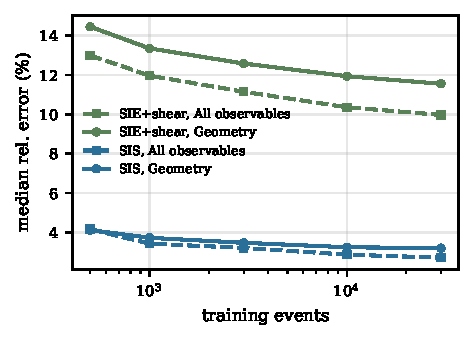
\includegraphics[width=\columnwidth]{fig_learning.pdf}
\caption{Median relative error of $\mu_A$ versus the number of training events for ET.}
\label{fig:learning}
\end{figure}


\section{Likelihoods of the Bayesian lens reconstruction}
\label{app:gwemlike}
This appendix specifies the analyses of Sec.~\ref{sec:gwem}. The lens parameters are $\boldsymbol\eta=(\sigma_v,x_c,y_c,q,\phi_q,\gamma_{\rm ext},\phi_{\rm ext},\gamma')$, with the subset appropriate to each lens model. Their priors are the simulated population distributions: the $\sigma_v^4$-weighted velocity-dispersion function on $100<\sigma_v<400$\,km\,s$^{-1}$, a Gaussian of width 0.02\,arcsec for the lens center relative to the observed light center, $q\sim\mathcal N(0.75,0.15)$ truncated to $[0.35,0.99]$, $\ln\gamma_{\rm ext}\sim\mathcal N(\ln0.05,0.6)$ truncated to $[\ln10^{-3},\ln0.25]$, $\gamma'\sim\mathcal N(2.08,0.15)$ truncated to $[1.6,2.6]$, and uniform position angles. The Einstein radius follows from $\sigma_v$ through the SIS relation at the observed redshifts.

\emph{EM likelihood.} Each observed image position $\boldsymbol\theta_i$, with uncertainty $\sigma_i$, maps to the source plane as $\boldsymbol\beta_i=\boldsymbol\theta_i-\boldsymbol\alpha(\boldsymbol\theta_i;\boldsymbol\eta)$. To first order, a source position $\boldsymbol\beta$ predicts an image displaced from $\boldsymbol\theta_i$ by $A_i^{-1}(\boldsymbol\beta_i-\boldsymbol\beta)$, where $A_i$ is the lensing Jacobian at $\boldsymbol\theta_i$, so that
\begin{equation}
\begin{split}
-2\ln\mathcal L_{\rm pos}(\boldsymbol\eta,\boldsymbol\beta)={}&\sum_i(\boldsymbol\beta_i-\boldsymbol\beta)^{\rm T}W_i(\boldsymbol\beta_i-\boldsymbol\beta)\\
&+\sum_i 2\ln(2\pi\sigma_i^2),
\end{split}
\end{equation}
with $W_i=A_i^{-\rm T}A_i^{-1}/\sigma_i^2$.
Integrating over $\boldsymbol\beta$ with a flat prior gives
\begin{equation}
\begin{split}
\ln\mathcal L_{\rm pos}(\boldsymbol\eta)={}&-\tfrac12\chi^2_{\rm min}-\tfrac12\ln\det W\\
&+\ln2\pi-\sum_i\ln(2\pi\sigma_i^2),
\end{split}
\end{equation}
with $W=\sum_iW_i$,
where $\chi^2_{\rm min}$ is evaluated at $\hat{\boldsymbol\beta}=W^{-1}\sum_iW_i\boldsymbol\beta_i$; the parameter-dependent normalization $-\frac12\ln\det W$ is retained. The model images are obtained by one Newton step from the observed positions, and the magnifications, Morse indices and Fermat potentials of the two GW images are evaluated there. In the exact variant, used as a check in Sec.~\ref{sec:gwem} and for coarse astrometry in Sec.~\ref{sec:discussion}, the source position is sampled as $\boldsymbol\beta=\hat{\boldsymbol\beta}+L\boldsymbol u$, with $LL^{\rm T}=W^{-1}$ and $\boldsymbol u$ uniform in $[-8,8]^2$; each model image is found by iterating the lens equation to convergence from the observed position, and $\ln\mathcal L_{\rm pos}=-\frac12\sum_i|\boldsymbol\theta_i^{\rm model}-\boldsymbol\theta_i|^2/\sigma_i^2-\sum_i\ln(2\pi\sigma_i^2)+\ln\det L$, where the last term makes the prior flat in $\boldsymbol\beta$. The EM likelihood multiplies $\mathcal L_{\rm pos}$ by Gaussians for the light axis ratio (width 0.05), the light position angle (width $10\degr$) and the measured velocity dispersion (width $0.1\sigma_v$).

\emph{Source-position prior.} A flat prior on $\boldsymbol\beta$ with the same normalization for every lens model does not reproduce the simulated population. The simulation draws the source uniformly in area within a disk of radius $R\,\theta_E$ ($R=1$ for the SIS, 1.6 for the SIE and 1.8 for the models with shear) and redraws it, up to 60 times, until the lens produces at least two images; after 60 failures the lens itself is redrawn. For a given lens the source density is therefore $1/A_{\rm mult}$ over the multiple-image region, the set of source positions that produce at least two images, whose area is $A_{\rm mult}=a\,\pi(R\theta_E)^2$, where $a(\boldsymbol\eta)$ is the fraction of the disk inside that region. The lens is retained with probability $1-(1-a)^{60}$. We therefore multiply the EM likelihood by $[1-(1-a)^{60}]/A_{\rm mult}$. The fraction $a$ is computed with the image solver and acceptance test of the simulation on a fixed set of 1200 source positions, tabulated on a grid in $\gamma'$, $q$, $\gamma_{\rm ext}$ and the angle between the shear and the mass major axis, and interpolated between grid points ($a=1$ for the SIS). Without this factor the posterior weights each lens model by $A_{\rm mult}$, which grows steeply with the slope. For $q=0.75$ and $\gamma_{\rm ext}=0.05$, $a=0.09$, 0.30 and 0.84 at $\gamma'=1.8$, 2.0 and 2.2, because a steeper profile forms a faint central image even for sources well outside the Einstein radius. The omission therefore favors steep slopes and underestimates $\mu_A$. We tested this on 143 EPL+shear systems drawn from the population without any detection requirement and analyzed with the EM data alone. Without the factor the posterior mean slope exceeds the true slope by $0.050\pm0.011$ on average, the median of $\ln\mu_A$ is low by $0.106\pm0.023$, and the 90\% credible intervals contain the true slope and $\mu_A$ in 87\% of the systems. With the factor the offsets are $-0.014\pm0.011$ and $-0.022\pm0.023$, the intervals contain the true values in 93\% and 90\%, and the fraction of posterior samples below the true value is consistent with a uniform distribution, as expected for calibrated posteriors (Kolmogorov--Smirnov $p=0.62$ for the slope and 0.98 for $\ln\mu_A$, compared with $p\le0.001$ without the factor). All results in Sec.~\ref{sec:gwem} include the factor.

\emph{GW quantities predicted by the lens.} For the known image assignment, the lens model predicts $\mu_A=|\mu_a|$, the ratio $R=|\mu_b/\mu_a|$, the Morse indices $n_A$, $n_B$, and the Fermat-potential difference $\Delta\phi$. Without a cosmology, the GW data constrain only $R$, $n_A$, $n_B$ and the arrival order: $\Delta\phi$ must have the sign of the measured delay, and the dimensional delay and the apparent distance remain free nuisance parameters.

\emph{Two-stage analysis.} The joint-PE posterior $p(\boldsymbol\xi|d)$, with GW parameters $\boldsymbol\xi$, is converted into an effective likelihood for the quantities the lens predicts, $\mathcal L_{\rm eff}(\ln R,\ln D_{{\rm app},A},n_A,n_B)\propto p(\ln R,\ln D_{{\rm app},A},n_A,n_B|d)/\pi_{\rm PE}$. The PE priors are uniform in $\ln R$ and in the Morse indices and $\propto D_{{\rm app},A}^2$ in distance; the other GW parameters (masses, spins, sky position, orientation, phase, arrival time and delay) are marginalized under their PE priors, which do not depend on the lens. We approximate $\mathcal L_{\rm eff}$ by a two-dimensional Gaussian in $(\ln R,\ln D_{{\rm app},A})$, fitted to the posterior samples with weights $D_{{\rm app},A}^{-3}$ (which remove the distance prior and convert to $\ln D$), multiplied by the marginal posterior probabilities of the nine Morse combinations, $P(n_A,n_B)=(k+0.5)/(N+4.5)$ for $k$ of $N$ samples. This product neglects any dependence of the $\ln R$ distribution on the Morse combination. In the PE posteriors the conditional means of $\ln R$ for different combinations differ from the overall mean by a median 0.03 (ET, host sky position) and 0.05 (O5) posterior standard deviations, with 90th percentiles of 0.08 and 0.19. Because no cosmology is assumed, only the $\ln R$ marginal is used.


\begin{thebibliography}{99}
\bibitem[Takahashi \& Nakamura(2003)]{takahashi2003waveeffects}
R. Takahashi and T. Nakamura, Astrophys. J. \textbf{595}, 1039 (2003).
\bibitem[Dai \& Venumadhav(2017)]{dai2017morse}
L. Dai and T. Venumadhav, arXiv:1702.04724.
\bibitem[Ezquiaga et al.(2021)]{ezquiaga2021phase}
J. M. Ezquiaga, D. E. Holz, W. Hu, M. Lagos, and R. M. Wald, Phys. Rev. D \textbf{103}, 064047 (2021).
\bibitem[Ng et al.(2018)]{ng2018rates}
K. K. Y. Ng, K. W. K. Wong, T. Broadhurst, and T. G. F. Li, Phys. Rev. D \textbf{97}, 023012 (2018).
\bibitem[Li et al.(2018)]{li2018statistical}
S.-S. Li, S. Mao, Y. Zhao, and Y. Lu, Mon. Not. R. Astron. Soc. \textbf{476}, 2220 (2018).
\bibitem[Oguri(2018)]{oguri2018distribution}
M. Oguri, Mon. Not. R. Astron. Soc. \textbf{480}, 3842 (2018).
\bibitem[Wierda et al.(2021)]{wierda2021beyond}
A. R. A. C. Wierda, E. Wempe, O. A. Hannuksela, L. V. E. Koopmans, and C. Van Den Broeck, Astrophys. J. \textbf{921}, 154 (2021).
\bibitem[Hannuksela et al.(2019)]{hannuksela2019search}
O. A. Hannuksela, K. Haris, K. K. Y. Ng, S. Kumar, A. K. Mehta, D. Keitel, T. G. F. Li, and P. Ajith, Astrophys. J. Lett. \textbf{874}, L2 (2019).
\bibitem[Abbott et al.(2021)]{lvk2021o3a}
R. Abbott \textit{et al.} (LIGO Scientific Collaboration and Virgo Collaboration), Astrophys. J. \textbf{923}, 14 (2021).
\bibitem[Abbott et al.(2024)]{lvk2024o3search}
R. Abbott \textit{et al.} (LIGO Scientific Collaboration, Virgo Collaboration and KAGRA Collaboration), Astrophys. J. \textbf{970}, 191 (2024).
\bibitem[LIGO Scientific Collaboration et al.(2025c)]{lvk2025gwtc4lensing}
LIGO Scientific, Virgo, and KAGRA Collaborations, arXiv:2512.16347.
\bibitem[LIGO Scientific Collaboration et al.(2025a)]{lvk2025gwtc4}
LIGO Scientific, Virgo, and KAGRA Collaborations, arXiv:2508.18082.
\bibitem[Liao et al.(2017)]{liao2017precision}
K. Liao, X.-L. Fan, X. Ding, M. Biesiada, and Z.-H. Zhu, Nat. Commun. \textbf{8}, 1148 (2017).
\bibitem[Oguri(2019)]{oguri2019review}
M. Oguri, Rep. Prog. Phys. \textbf{82}, 126901 (2019).
\bibitem[Hannuksela et al.(2020)]{hannuksela2020localizing}
O. A. Hannuksela, T. E. Collett, M. {\c{C}}al{\i}{\c{s}}kan, and T. G. F. Li, Mon. Not. R. Astron. Soc. \textbf{498}, 3395 (2020).
\bibitem[Wempe et al.(2024)]{wempe2022lensing}
E. Wempe, L. V. E. Koopmans, A. R. A. C. Wierda, O. A. Hannuksela, and C. Van Den Broeck, Mon. Not. R. Astron. Soc. \textbf{530}, 3368 (2024).
\bibitem[Smith et al.(2023)]{smith2023discovering}
G. P. Smith \textit{et al.}, Mon. Not. R. Astron. Soc. \textbf{520}, 702 (2023).
\bibitem[Uronen et al.(2026b)]{uronen2026galacticcentres}
L. Uronen, T. Li, Q. He, J. Janquart, T. Collett, L. V. E. Koopmans, and O. Hannuksela, arXiv:2609.10285.
\bibitem[Falco, Gorenstein \& Shapiro(1985)]{falco1985msd}
E. E. Falco, M. V. Gorenstein, and I. I. Shapiro, Astrophys. J. Lett. \textbf{289}, L1 (1985).
\bibitem[Schneider \& Sluse(2013)]{schneider2013msd}
P. Schneider and D. Sluse, Astron. Astrophys. \textbf{559}, A37 (2013).
\bibitem[Poon et al.(2025)]{poon2025degeneracy}
J. S. C. Poon, S. Rinaldi, J. Janquart, H. Narola, and O. A. Hannuksela, Mon. Not. R. Astron. Soc. \textbf{536}, 2212 (2025).
\bibitem[Uronen et al.(2026a)]{uronen2026silmarel}
L. Uronen \textit{et al.}, arXiv:2603.09794.
\bibitem[Meneghetti et al.(2017)]{meneghetti2017ff}
M. Meneghetti \textit{et al.}, Mon. Not. R. Astron. Soc. \textbf{472}, 3177 (2017).
\bibitem[LIGO Scientific Collaboration et al.(2025b)]{lvk2025gwtc4pop}
LIGO Scientific, Virgo, and KAGRA Collaborations, arXiv:2508.18083.
\bibitem[Schneider, Ehlers \& Falco(1992)]{schneider1992gravitationallenses}
P. Schneider, J. Ehlers, and E. E. Falco, \textit{Gravitational Lenses} (Springer-Verlag, Berlin, 1992).
\bibitem[Madau \& Dickinson(2014)]{madau2014cosmic}
P. Madau and M. Dickinson, Annu. Rev. Astron. Astrophys. \textbf{52}, 415 (2014).
\bibitem[Turner, Ostriker \& Gott(1984)]{turner1984statistics}
E. L. Turner, J. P. Ostriker, and J. R. Gott, Astrophys. J. \textbf{284}, 1 (1984).
\bibitem[Choi, Park \& Vogeley(2007)]{choi2007vdf}
Y.-Y. Choi, C. Park, and M. S. Vogeley, Astrophys. J. \textbf{658}, 884 (2007).
\bibitem[Bolton et al.(2008)]{bolton2008slacs}
A. S. Bolton, S. Burles, L. V. E. Koopmans, T. Treu, R. Gavazzi, L. A. Moustakas, R. Wayth, and D. J. Schlegel, Astrophys. J. \textbf{682}, 964 (2008).
\bibitem[Auger et al.(2010)]{auger2010slacs}
M. W. Auger, T. Treu, A. S. Bolton, R. Gavazzi, L. V. E. Koopmans, P. J. Marshall, L. A. Moustakas, and S. Burles, Astrophys. J. \textbf{724}, 511 (2010).
\bibitem[Tessore \& Metcalf(2015)]{tessore2015epl}
N. Tessore and R. B. Metcalf, Astron. Astrophys. \textbf{580}, A79 (2015).
\bibitem[Birrer \& Amara(2018)]{birrer2018lenstronomy}
S. Birrer and A. Amara, Phys. Dark Universe \textbf{22}, 189 (2018).
\bibitem[Birrer et al.(2021)]{birrer2021lenstronomy}
S. Birrer \textit{et al.}, J. Open Source Softw. \textbf{6}, 3283 (2021).
\bibitem[Hild et al.(2011)]{hild2011etd}
S. Hild \textit{et al.}, Classical Quantum Gravity \textbf{28}, 094013 (2011).
\bibitem[Pratten et al.(2020)]{pratten2020xas}
G. Pratten, S. Husa, C. Garc{\'i}a-Quir{\'o}s, M. Colleoni, A. Ramos-Buades, H. Estell{\'e}s, and R. Jaume, Phys. Rev. D \textbf{102}, 064001 (2020).
\bibitem[Haris et al.(2018)]{haris2018identifying}
K. Haris, A. K. Mehta, S. Kumar, T. Venumadhav, and P. Ajith, arXiv:1807.07062.
\bibitem[Planck Collaboration(2020)]{planck2020cosmology}
Planck Collaboration, Astron. Astrophys. \textbf{641}, A6 (2020).
\bibitem[Janquart et al.(2023)]{janquart2023golum}
J. Janquart, K. Haris, O. A. Hannuksela, and C. Van Den Broeck, Mon. Not. R. Astron. Soc. \textbf{526}, 3088 (2023).
\bibitem[Lo \& Maga{\~n}a Hernandez(2023)]{lo2023bayesian}
R. K. L. Lo and I. Maga{\~n}a Hernandez, Phys. Rev. D \textbf{107}, 123015 (2023).
\bibitem[Abbott et al.(2023)]{gwosc2023}
R. Abbott \textit{et al.} (LIGO Scientific Collaboration, Virgo Collaboration and KAGRA Collaboration), Astrophys. J. Suppl. Ser. \textbf{267}, 29 (2023).
\bibitem[Cutler \& Flanagan(1994)]{cutler1994gravitational}
C. Cutler and {\'E}. E. Flanagan, Phys. Rev. D \textbf{49}, 2658 (1994).
\bibitem[Pedregosa et al.(2011)]{pedregosa2011scikit}
F. Pedregosa \textit{et al.}, J. Mach. Learn. Res. \textbf{12}, 2825 (2011).
\bibitem[Romano, Patterson \& Cand{\`e}s(2019)]{romano2019cqr}
Y. Romano, E. Patterson, and E. Cand{\`e}s, in \textit{Advances in Neural Information Processing Systems 32} (Curran Associates, Red Hook, NY, 2019), p.~3543.
\bibitem[Vovk, Gammerman \& Shafer(2005)]{vovk2005algorithmic}
V. Vovk, A. Gammerman, and G. Shafer, \textit{Algorithmic Learning in a Random World} (Springer, New York, 2005).
\bibitem[Papamakarios \& Murray(2016)]{papamakarios2016fast}
G. Papamakarios and I. Murray, in \textit{Advances in Neural Information Processing Systems 29} (Curran Associates, Red Hook, NY, 2016), p.~1028.
\bibitem[Dax et al.(2021)]{dax2021neuralposterior}
M. Dax, S. R. Green, J. Gair, J. H. Macke, A. Buonanno, and B. Sch{\"o}lkopf, Phys. Rev. Lett. \textbf{127}, 241103 (2021).
\bibitem[Durkan et al.(2019)]{durkan2019nsf}
C. Durkan, A. Bekasov, I. Murray, and G. Papamakarios, in \textit{Advances in Neural Information Processing Systems 32} (Curran Associates, Red Hook, NY, 2019), p.~7511.
\bibitem[Rozet et al.(2022)]{rozet2022zuko}
F. Rozet \textit{et al.}, zuko: Normalizing flows in PyTorch, Zenodo (2022), doi:10.5281/zenodo.7625672.
\bibitem[Wagner-Carena et al.(2021)]{wagnercarena2021hierarchical}
S. Wagner-Carena, J. W. Park, S. Birrer, P. J. Marshall, A. Roodman, and R. H. Wechsler, Astrophys. J. \textbf{909}, 187 (2021).
\bibitem[Park et al.(2021)]{park2021largescale}
J. W. Park, S. Wagner-Carena, S. Birrer, P. J. Marshall, J. Y.-Y. Lin, and A. Roodman, Astrophys. J. \textbf{910}, 39 (2021).
\bibitem[Liu et al.(2024)]{liu2024harmonics}
J.-D. Liu, W.-B. Han, Q. Yun, and S.-C. Yang, arXiv:2405.11279.
\bibitem[Garc{\'\i}a-Quir{\'o}s et al.(2020)]{garciaquiros2020xhm}
C. Garc{\'\i}a-Quir{\'o}s \textit{et al.}, Phys. Rev. D \textbf{102}, 064002 (2020).
\bibitem[Ashton et al.(2019)]{ashton2019bilby}
G. Ashton \textit{et al.}, Astrophys. J. Suppl. Ser. \textbf{241}, 27 (2019).
\bibitem[Speagle(2020)]{speagle2020dynesty}
J. S. Speagle, Mon. Not. R. Astron. Soc. \textbf{493}, 3132 (2020).
\bibitem[Zackay, Dai \& Venumadhav(2018)]{zackay2018relbin}
B. Zackay, L. Dai, and T. Venumadhav, arXiv:1806.08792.
\bibitem[Krishna et al.(2023)]{krishna2023relbin}
K. Krishna \textit{et al.}, arXiv:2312.06009.
\end{thebibliography}


\end{document}
